% ============================================================================
% arXiv preprint wrapper for the shared manuscript body.
% ============================================================================
\documentclass[11pt]{article}

\usepackage[letterpaper,margin=1in]{geometry}
\usepackage[utf8]{inputenc}
\usepackage[T1]{fontenc}
\usepackage{mathptmx}
\usepackage{url}
\usepackage{microtype}
\usepackage{amsmath}
\usepackage{amssymb}
\usepackage{bm}
\usepackage{amsthm}
\usepackage{algorithm}
\usepackage{algorithmic}
\usepackage{array}
\usepackage{booktabs}
\usepackage{graphicx}
\usepackage{subcaption}
\usepackage{xcolor}
\usepackage[hidelinks,hypertexnames=false,bookmarks=false]{hyperref}
\graphicspath{{figures/}{./figures/}}

\newtheorem{theorem}{Theorem}
\newtheorem{proposition}{Proposition}
\newtheorem{lemma}{Lemma}
\newtheorem{definition}{Definition}
\newtheorem{remark}{Remark}
\newtheorem{corollary}{Corollary}

\DeclareMathOperator*{\argmax}{arg\,max}
\DeclareMathOperator*{\argmin}{arg\,min}
\DeclareMathOperator{\Var}{Var}
\DeclareMathOperator{\Cov}{Cov}
\DeclareMathOperator{\tr}{tr}

\newcolumntype{L}[1]{>{\raggedright\arraybackslash}p{#1}}

\newcommand{\answerYes}[1][]{[Yes]#1}
\newcommand{\answerNo}[1][]{[No]#1}
\newcommand{\answerNA}[1][]{[N/A]#1}

\title{\Large\bfseries Path-Gain Compressibility Determines\\Local Credit Assignment in Conductance-Based Dendrites}
\author{%
  Author One$^{1}$, \quad
  Author Two$^{1,2}$, \quad
  Corresponding Author$^{1}$\thanks{Corresponding author: \href{mailto:email@example.org}{email@example.org}} \\
  $^{1}$Affiliation One \qquad $^{2}$Affiliation Two
}
\date{\today}

\begin{document}
\maketitle

% Shared manuscript body lives in local_credit_assignment_body.tex.
\begin{abstract}
Biological neurons assign credit through structures that standard neural networks usually ignore: synapses are distributed across branching dendrites, inputs arrive as excitatory and inhibitory conductances, and inhibition can shunt local voltage by changing input resistance. We study conductance-based dendritic networks with E/I synapse banks, shunting integration, and tree-structured branch-to-soma coupling, and ask when a low-bandwidth somatic broadcast can replace the compartment-specific errors of backpropagation. Exact gradients for this conductance tree show that each synaptic update separates into a local eligibility term built from presynaptic activity, driving force, and input resistance, and one non-local compartment error. Under identity upward transfer, that error is the somatic error transported through conductance-stage path gains. This factorization turns local learning into a credit-signal compression problem: broadcast is useful only when it approximates the path-specific compartment-error field. We test this mechanism across gradient, oracle-transport, inhibition-intervention, competence, morphology, and harder-data diagnostics. Shunting improves LocalCA--backprop alignment, reduces gradient-scale mismatch, and makes exact compartment errors more rank-1 compressible than matched additive controls in the regimes studied here. Inhibitory-conductance interventions show that learned inhibition carries sample-specific pathway structure, while transported-error oracle experiments show that restoring the exact path-gain error largely closes the local-learning gap. Under nonnegative conductances and rank-1 broadcast, shunting LocalCA remains within about 5--6 percentage points of matched backpropagation reference performance on MNIST, Fashion-MNIST, and context gating. These results suggest that E/I conductance, shunting inhibition, and dendritic branching can reshape credit-signal geometry and make low-bandwidth local learning more faithful.
\end{abstract}

%=============================================================================
\section{Introduction}
\label{sec:intro}
%=============================================================================

Unlike point units in standard neural networks, biological neurons assign credit across branching dendritic trees. A synapse does not only see presynaptic activity and a scalar postsynaptic activation; it also has access to local membrane voltage, synaptic reversal potential, total conductance, and input resistance. Inhibitory input can therefore do more than subtract activity: by increasing local conductance, it can shunt voltage and change the gain of every dendritic path passing through that compartment.

We ask whether these biophysical ingredients can make local credit assignment easier. Backpropagation would assign a distinct error to every dendritic compartment, whereas a biologically plausible supervisory signal is more likely to arrive as a low-bandwidth somatic or modulatory broadcast \cite{richards2019dendritic}. The central question is therefore not whether such a broadcast can reproduce unconstrained backpropagation in every setting, but when the exact dendritic error field is simple enough for it to approximate.
Our contribution is not simply to add dendritic structure to a neural network, but to show how conductance, shunting inhibition, and dendritic topology change the geometry of the credit signal itself.

\begin{figure}[!t]
\centering
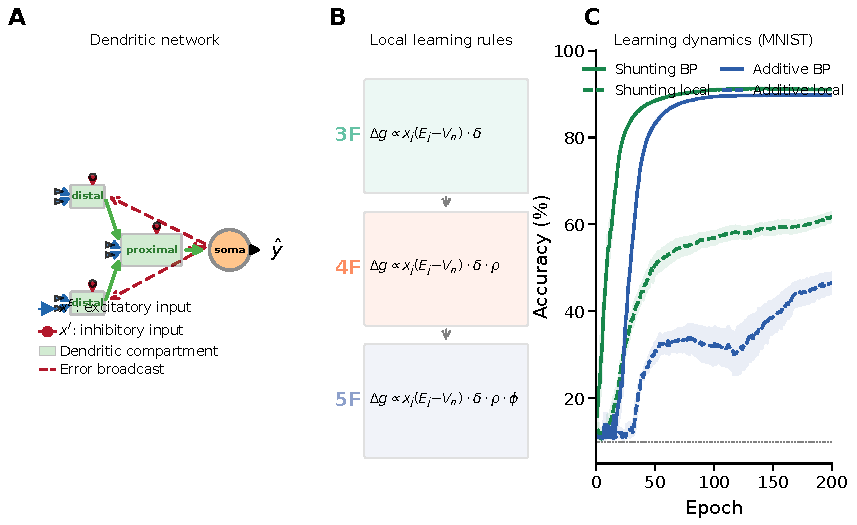
\includegraphics[width=\textwidth]{fig1_model_and_credit.pdf}
\caption{\textbf{Model and credit assignment.}
\textbf{(A)}~Conductance tree with nonnegative excitatory drive and inhibitory shunting load.
\textbf{(B)}~Exact credit varies by dendritic path, whereas rank-1 LocalCA broadcasts one shared error field.
\textbf{(C)}~LocalCA preserves the exact synapse-local eligibility and substitutes $e_n\!\approx\!\delta_n$; rank-1, neuron-wise, rank-$K$, and path-structured broadcasts trade biological bandwidth for fidelity, while transported error is an oracle.}
\label{fig:model_schematic}
\end{figure}

Starting from conductance-based dendritic voltage equations \cite{koch1999biophysics}, we derive exact gradients for dendritic trees (Theorem~\ref{thm:tree_backprop}). Each synaptic gradient factorizes into a synapse-local eligibility term and a single non-local compartment error. The eligibility term depends on presynaptic activity, driving force, and input resistance. The compartment error is path-specific: under identity upward transfer it is the somatic error multiplied by a conductance-stage path gain through the dendritic tree. LocalCA preserves the exact local eligibility and replaces this path-specific error with a broadcast field.

This factorization turns local credit assignment into a compressibility problem. By compressibility, we mean that the matrix of exact compartment errors across examples and compartments is well approximated by a low-rank signal, especially a rank-1 field shared across compartments. Dendritic branching creates the paths; E/I synapse banks set the local conductance state; and shunting inhibition changes the input resistance along each path. Shunting is not assumed to help monotonically. It helps rank-1 broadcast when inhibitory conductance attenuates high-gain paths or otherwise makes the exact error field more compressible.

\paragraph{Related work.}
This work builds on models of dendritic integration, branch-level nonlinear computation, normalization, and biologically plausible teaching signals \cite{koch1983nonlinear,koch1999biophysics,poiarazi2003pyramidal,london2005dendritic,silver2010neuronal,carandini2012normalization,urbanczik2014dendritic,guerguiev2017segregated,sacramento2018dendritic,whittington2019theories,payeur2021burst,greedy2022burstccn,haider2021latent,song2024prospective,iyer2022activedendrites}.
It also connects to machine-learning approaches that replace exact backpropagation with local, random, predictive, equilibrium, perturbation, or broadcast feedback signals \cite{lillicrap2016random,nokland2016dfa,lee2015dtp,scellier2017equilibrium,meulemans2021dfc,millidge2022predictive,hinton2022forward,dellaferrera2022pepita,pal2024local,ma2024auglocal,lv2025dll,erdogan2025ebd,kao2024ccl}.
Our contribution is complementary: we derive the exact conductance-tree credit object and test when shunting inhibition and dendritic morphology make that object broadcast-compatible.

We test this chain directly. Exact-gradient reconstruction verifies the factorization numerically. Gradient-fidelity diagnostics show that shunting produces local updates that are better aligned and better scaled relative to backpropagation than matched additive controls. Exact-error compressibility and inhibition-intervention diagnostics show that learned inhibitory conductance carries sample-specific pathway structure. Transported-error oracle experiments show that supplying the exact path-gain-transported compartment error largely closes the local-learning gap, identifying broadcast fidelity as the main bottleneck. In an MNIST gradient-dynamics diagnostic, shunting improves final local-backprop alignment (cosine $0.100\pm0.033$ vs.\ $0.005\pm0.026$) and reduces scale mismatch ($0.26\pm0.05$ vs.\ $0.50\pm0.05$). On noise resilience under matched inhibition ($N_I \geq 5$), transported error raises additive local learning from $81$--$84\%$ under rank-1 broadcast to $92$--$94\%$, nearly matching shunting at $95$--$95.2\%$.

\paragraph{Contributions.}
This paper makes three contributions. First, we derive the exact gradient for a conductance-based dendritic tree and show that synaptic credit separates into a local eligibility term and a path-specific compartment error. Second, we identify path-gain compressibility as the quantity that mediates whether a low-rank somatic broadcast can approximate this error. Third, we show empirically that shunting inhibition can improve this approximation by changing input resistance along dendritic paths, while also identifying regimes where rank-1 feedback fails and richer pathway-specific feedback is needed.

\begin{figure}[!t]
\centering
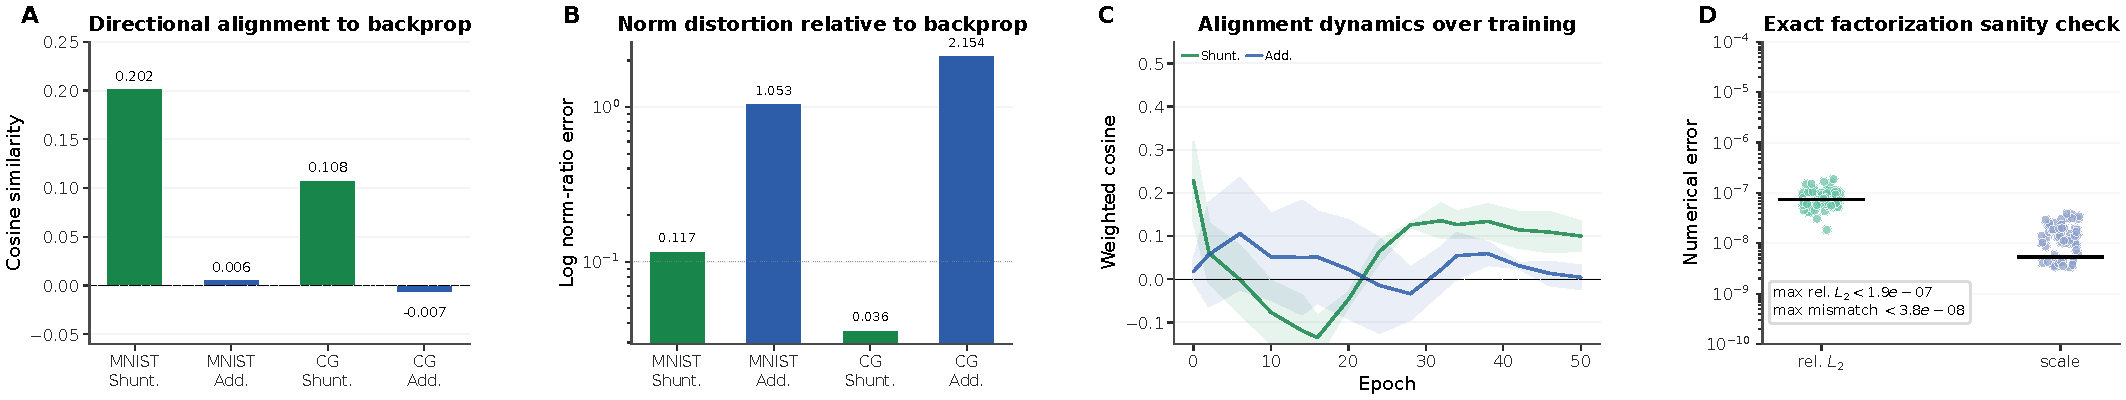
\includegraphics[width=\textwidth]{fig3_gradient_fidelity.pdf}
\caption{\textbf{Gradient-fidelity diagnostic.} \textbf{(A)}~Exact-factorization sanity check: reconstructed gradients match autograd to numerical precision. \textbf{(B)}~Final-state weighted cosine similarity between local and backprop gradients. \textbf{(C)}~Final-state scale mismatch, $|\log_{10}(\|g^{\mathrm{local}}\|/\|g^{\mathrm{bp}}\|)|$. Error bars are $\pm$1 s.d.\ across 3 gradient-dynamics seeds; main learning and oracle sweeps use 5 seeds unless noted. \textbf{(D)}~Alignment over learning; Appendix Fig.~\ref{fig:alignment_norm_dynamics} shows finite gradient norms.}
\label{fig:gradient_fidelity}
\end{figure}

%=============================================================================
\section{Compartmental Voltage Model and Gradient Derivation}
\label{sec:model}
%=============================================================================

We use a steady-state conductance model derived from discretized passive cable dynamics \cite{koch1999biophysics,dayan2001theoretical}.
In normalized units, leak and inhibitory reversal are set to $0$, the excitatory reversal is set to $1$, and leak conductance is fixed at $1$.
Each compartment computes a conductance-weighted voltage: excitatory conductance pulls the voltage toward the excitatory reversal potential, leak and shunting inhibition pull it toward zero, and dendritic coupling transfers child voltages upward toward the soma. This form makes local sensitivity depend on both driving force $(E{-}V)$ and total input resistance $R^{\mathrm{tot}}$.
Throughout the paper we write dendritic morphologies as rooted trees $[b_1,b_2,\dots,b_D]$, where each factor gives the fan-in from one dendritic stage to the next on the path to the soma. Thus $[3,3]$ means that each soma aggregates $3$ proximal branches and each proximal branch aggregates $3$ distal branches, for $9$ distal leaves per soma. In the main feedforward experiments, synaptic inputs terminate on dendritic branches rather than directly on the soma. Each branch layer carries explicit excitatory conductance banks and, when enabled, learned inhibitory branch-level conductance banks driven by nonnegative inputs. This is input-driven shunting inhibition, not a recurrent lateral inhibitory circuit; explicit inhibitory-cell controls are reported in the appendix. The additive and shunting cores are architecture-matched at the tree level and differ only in the branch-level voltage integration rule.
These ingredients play distinct roles in the credit-assignment argument. Branching creates the path structure. E/I synapse banks determine the local conductance state. Shunting turns inhibitory conductance into a multiplicative change in input resistance. The local learning rule then asks whether a low-bandwidth teaching signal can stand in for the exact path-specific error induced by that tree.
\paragraph{Notation.}
We use $\alpha_n$ for the exact conductance-stage path gain from compartment $n$ to the soma, $r_n^{\mathrm{4F}}$ for the empirical 4F branch-soma covariance proxy, $\phi_n$ for the 5F confidence factor, $\lambda_{\mathrm{mix}}$ for the pathway-broadcast mixing weight, and $\kappa_j$ for depth-dependent modulation in morphology extensions.
All conductances and presynaptic activities in the main experimental setting are nonnegative; additive voltages may be signed comparators, but the conductance variables that define the shunting model are nonnegative.

\subsection{Voltage Equation and Local Sensitivities}

Consider compartment $n$ with synaptic inputs $j$ (activity $x_j$, reversal $E_j$, conductance $g_j^{\mathrm{syn}}\!\geq\!0$) and dendritic inputs from children (voltage $V_j$, conductance $g_j^{\mathrm{den}}\!\geq\!0$).
The steady-state voltage is:
\begin{equation}
V_n = \frac{\sum_j E_j x_j g_j^{\mathrm{syn}} + \sum_j V_j g_j^{\mathrm{den}}}{\underbrace{\sum_j x_j g_j^{\mathrm{syn}} + \sum_j g_j^{\mathrm{den}} + 1}_{g_n^{\mathrm{tot}}}},
\qquad R_n^{\mathrm{tot}} = 1/g_n^{\mathrm{tot}}.
\label{eq:voltage}
\end{equation}
$V_n$ is a convex combination of reversal potentials, child voltages, and leak. Writing $\mathcal{S}_n = \{0\} \cup \{E_j\}_j \cup \{V_j\}_j$, we have $\min\mathcal{S}_n \leq V_n \leq \max\mathcal{S}_n$ and $0 < R_n^{\mathrm{tot}} \leq 1$.
The local sensitivities follow directly:

\begin{proposition}[Local Sensitivities]
\label{prop:sensitivities}
\begin{equation}
\frac{\partial V_n}{\partial g_i^{\mathrm{syn}}} = x_i R_n^{\mathrm{tot}} (E_i - V_n),
\quad
\frac{\partial V_n}{\partial V_i} = g_i^{\mathrm{den}} R_n^{\mathrm{tot}},
\quad
\frac{\partial V_n}{\partial g_i^{\mathrm{den}}} = R_n^{\mathrm{tot}} (V_i - V_n).
\label{eq:sensitivities}
\end{equation}
\end{proposition}
Eq.~\eqref{eq:sensitivities} gives the eligibility factors used by the local rules below: presynaptic activity or voltage difference, driving force, and input resistance.

\subsection{Shunting Inhibition as Divisive Gain Control}

An inhibitory synapse with $E_{\mathrm{inh}}\!\approx\!0$ contributes current $(0{-}V_n)x_j g_j^{\mathrm{syn}}$ and increases $g_n^{\mathrm{tot}}$.
Its sensitivity is $\partial V_n / \partial g_j^{\mathrm{syn}} = -x_j R_n^{\mathrm{tot}} V_n$, which corresponds to multiplicative attenuation (divisive normalization).
Shunting is divisive at the voltage level, but its effect on firing rates can be subtractive in some regimes \cite{holt1997shunting}.
Inhibitory plasticity can balance excitation dynamically \cite{vogels2011inhibitory}; our learned inhibitory conductances serve an analogous role.
The same denominator also gives the direct connection to path gain. Writing $G_n^E(x)$ and $G_n^I(x)$ for the total excitatory and inhibitory synaptic conductance impinging on compartment $n$,
\[
R_n^{\mathrm{tot}}(x)=\left(1+G_n^E(x)+G_n^I(x)+G_n^{\mathrm{den}}\right)^{-1}.
\]
Increasing $G_n^I(x)$ lowers $R_n^{\mathrm{tot}}(x)$ and therefore multiplicatively suppresses every upstream path whose error must pass through compartment $n$.
In this sense inhibition can gate credit flow by changing the path gain, even when the inhibitory drive is feedforward rather than lateral. Prop.~\ref{prop:inhibitory_path_gain} formalizes this statement after the tree path gain is defined.

\subsection{Exact Gradients for Dendritic Trees}

Let $V_0$ be the somatic output and define the soma/core error as $\delta_0 := \partial L / \partial V_0$.
For a linear decoder $\hat{y}=W_{\mathrm{dec}}V_0$, this reduces to $\delta_0 = W_{\mathrm{dec}}^\top(\partial L/\partial \hat{y})$; for a nonlinear decoder, $\delta_0$ is the corresponding decoder-input Jacobian product.
The theoretical derivation is stated for the conductance-stage voltage before any post-voltage reactivation. When a branch applies a monotone reactivation before transmitting activity upward, the same recursion holds with additional local derivative factors along the path. All exact-error diagnostics below are computed on pre-reactivation voltages, so they test the conductance-stage quantity derived here.

\begin{theorem}[Conductance-Stage Backpropagation on a Dendritic Tree]
\label{thm:tree_backprop}
For a rooted dendritic tree with soma at node $0$ and unique parent $p(n)$ for each non-somatic compartment, suppose the parent receives either the pre-reactivation voltage $V_n$ or a local post-voltage activity $a_n=f_n(V_n)$. For identity upward transfer, the loss gradient satisfies
\begin{equation}
\frac{\partial L}{\partial V_n}
= \frac{\partial L}{\partial V_{p(n)}}\, R_{p(n)}^{\mathrm{tot}}\, g_{n\to p(n)}^{\mathrm{den}},
\label{eq:tree_recursion}
\end{equation}
with boundary condition $\partial L / \partial V_0 = \delta_0$. With post-voltage transfer $a_n=f_n(V_n)$, the local factor becomes $f_n'(V_n)R_{p(n)}^{\mathrm{tot}}g_{n\to p(n)}^{\mathrm{den}}$. Because the graph is a tree, each compartment has a unique path to the soma. Defining the conductance-stage path gain
\begin{equation}
\alpha_n
= \prod_{(i\to k)\in \mathrm{path}(n\leadsto 0)} R_k^{\mathrm{tot}}\, g_{i\to k}^{\mathrm{den}},
\qquad
\frac{\partial L}{\partial V_n} = \alpha_n \delta_0,
\label{eq:path_sum}
\end{equation}
with $\alpha_0 = 1$ under identity transfer. In the post-voltage case, the exact effective path gain is obtained by multiplying the same product by the local factors $f_i'(V_i)$ on the transmitted child activities along the path.
\end{theorem}
\begin{proof}
Apply the chain rule on the tree-structured computation graph using Prop.~\ref{prop:sensitivities}.
\end{proof}
The one-step recursion in Eq.~\eqref{eq:tree_recursion} and the path product in Eq.~\eqref{eq:path_sum} separate local conductance transfer from the non-local somatic error.

\begin{proposition}[Inhibitory control of conductance-stage path gain]
\label{prop:inhibitory_path_gain}
Let $\mathcal{A}(n)$ be the set of compartments on the path from compartment $n$ to the soma, excluding $n$ and including the parent compartments through which the error must pass. Holding dendritic coupling conductances fixed, an added inhibitory conductance $\Delta G_k^I(x)\geq 0$ at any $k\in\mathcal{A}(n)$ changes the conductance-stage path gain by
\begin{equation}
\frac{\alpha_n(x;\Delta G^I)}{\alpha_n(x;0)}
=
\prod_{k\in\mathcal{A}(n)}
\frac{g_k^{\mathrm{tot}}(x)}
{g_k^{\mathrm{tot}}(x)+\Delta G_k^I(x)} ,
\qquad
\frac{\partial \log \alpha_n}{\partial G_k^I} =
\begin{cases}
-R_k^{\mathrm{tot}}, & k\in\mathcal{A}(n),\\
0, & k\notin\mathcal{A}(n).
\end{cases}
\label{eq:inhibition_path_gain_ratio}
\end{equation}
\end{proposition}
\begin{proof}
Substitute $R_k^{\mathrm{tot}}=1/g_k^{\mathrm{tot}}$ into the path-gain product in Eq.~\eqref{eq:path_sum}. Adding inhibitory conductance changes only the denominator at compartments on the path from $n$ to the soma, which gives the product ratio and the log derivative in Eq.~\eqref{eq:inhibition_path_gain_ratio}.
\end{proof}

Prop.~\ref{prop:inhibitory_path_gain} makes two directed predictions. First, inhibition is a path gate: it attenuates all credit paths below the inhibited compartment. Second, inhibition is useful for rank-$1$ local learning only when this attenuation makes the distribution of $\alpha_n$ more uniform or better aligned with the task. If inhibition is too strong, too heterogeneous, or generated by a poorly calibrated inhibitory population, it can suppress useful signals and hurt learning. In the additive control the same I input changes voltages and local eligibilities, but it does not enter the conductance-stage path recursion as a multiplicative resistance gate.

\paragraph{When does shunting compress path gains?}
The attenuation identity above is not by itself a concentration result. Let $z_n=\log \alpha_n$ be the log path gain for compartment $n$. If added inhibitory conductance contributes a path-dependent attenuation
\begin{equation}
\beta_n(x)=\sum_{k\in\mathcal{A}(n)}
\log\!\left(1+\frac{\Delta G_k^I(x)}{g_k^{\mathrm{tot}}(x)}\right),
\qquad
z'_n=z_n-\beta_n,
\label{eq:log_gain_attenuation}
\end{equation}
then, over compartments or examples,
\begin{equation}
\Var(z')=\Var(z)+\Var(\beta)-2\Cov(z,\beta).
\label{eq:log_gain_variance}
\end{equation}
Thus shunting narrows the log path-gain field exactly when
\begin{equation}
\Cov(z,\beta)>\frac{1}{2}\Var(\beta).
\label{eq:compression_condition}
\end{equation}
Eq.~\eqref{eq:log_gain_attenuation} follows by taking the logarithm of the product ratio in Prop.~\ref{prop:inhibitory_path_gain}; Eq.~\eqref{eq:log_gain_variance} then applies the variance identity for $z-\beta$. Eq.~\eqref{eq:compression_condition} is an interpretive sufficient condition under the same averaging measure, not a primary empirical diagnostic. In finite trained networks, the covariance margin can disagree with CV and exact-error-rank summaries because these statistics average over different compartment and sample axes. We therefore use direct path-gain dispersion, exact-error compressibility, and inhibition-intervention measurements as the empirical tests, and report the covariance margin as a boundary check in the appendix.

\begin{corollary}[Local--Global Factorization]
\label{cor:factorization}
The exact synaptic gradient at compartment $n$ factorizes as:
\begin{equation}
\frac{\partial L}{\partial g_i^{\mathrm{syn}}} =
\underbrace{x_i\, R_n^{\mathrm{tot}}\, (E_i - V_n)}_{\text{synapse-local eligibility}} \;\cdot\;
\underbrace{\frac{\partial L}{\partial V_n}}_{\text{compartment error}},
\label{eq:factorization}
\end{equation}
where the eligibility term depends only on quantities available at synapse $i$ (presynaptic activity $x_i$, input resistance $R_n^{\mathrm{tot}}$, driving force $E_i - V_n$), and the compartment error $\partial L / \partial V_n$ is the sole non-local quantity.
\end{corollary}
The factorization in Eq.~\eqref{eq:factorization} isolates the only non-local quantity as $\partial L / \partial V_n = \alpha_n \delta_0$ under identity upward transfer. With post-voltage transfer, the activation-derivative factors in Theorem~\ref{thm:tree_backprop} enter the effective path gain, but the compartment error remains the only non-local term. Any practical local rule therefore depends entirely on how well a broadcast signal approximates that exact compartment error, which we evaluate in Sec.~\ref{sec:grad_fidelity}.
In the models studied here, shunting improves this approximation by reducing and stabilizing $R_n^{\mathrm{tot}}$, which narrows the spread of local sensitivities across the tree.
In the empirical networks, each dendritic branch layer may optionally apply a post-voltage reactivation $f(V_n)$ before passing activity to the next stage; unless otherwise noted, the manuscript sweeps use a learnable bounded \texttt{param\_tanh} reactivation.

%=============================================================================
\section{Local Learning Rules}
\label{sec:local_rules}
%=============================================================================

\subsection{Broadcast Error Approximation}

We approximate the exact compartment error $\partial L / \partial V_n$ (Corollary~\ref{cor:factorization}) with a broadcast signal $e_n$ derived from the somatic/core error $\delta_0$. For a linear readout this reduces to $\delta_0 = W_{\mathrm{dec}}^\top (\partial L / \partial \hat{y})$; for a nonlinear decoder we use the corresponding decoder-input Jacobian product $J_{\mathrm{dec}}(h_{\mathrm{core}})^\top (\partial L / \partial \hat{y})$ so that the broadcast remains defined in the same core-space coordinates.
We distinguish five feedback objects:
\begin{itemize}
\item \textbf{Rank-1 shared broadcast:} $e_n = \bar{\delta}\cdot\mathbf{1}$, where $\bar{\delta} = \mathrm{mean}(\delta_0)$ is one scalar field delivered to all compartments.
\item \textbf{Neuron-wise broadcast:} $e_n = \delta_0$ when the layer width matches the core/output error dimension. In our main feedforward settings this condition usually fails, so the default neuron-wise implementation reduces to rank-1 shared broadcast.
\item \textbf{Rank-$K$ random broadcast:} $c = P_K\delta_0 \in \mathbb{R}^K$ and $e_n = \sum_{k=1}^{K} q_{n,k}c_k$, where $P_K$ is a fixed random projection and $q_{n,k}$ mixes those $K$ channels into compartment $n$.
\item \textbf{Path-structured broadcast:} $e_n = \lambda_{\mathrm{mix}}\,\bar{\delta}\cdot\mathbf{1} + (1{-}\lambda_{\mathrm{mix}})\,\Gamma_n(\delta_0)$, where $\Gamma_n$ projects the somatic error into router-inferred pathway roles, gates those roles by local pathway activity, and transports the resulting vector hierarchically through the block-structured dendritic tree \cite{nature2026vectorized}.
\item \textbf{Transported oracle:} $e_n^{\mathrm{transport}} = \alpha_n\delta_0 = \partial L/\partial V_n$. This is an analysis upper bound, not a proposed local rule, because it supplies the exact path gain $\alpha_n$ from Theorem~\ref{thm:tree_backprop}.
\end{itemize}
In the main feedforward architectures, hidden widths exceed the decoder-error dimension, so the default neuron-wise broadcast reduces to a rank-1 shared field (Appendix Table~\ref{tab:effective_broadcast_dimensionality}). Thus the main rank-1 result should be read as the architecture-induced low-bandwidth case, not as a claim that neuron-wise broadcasts were unavailable in principle. Under shunting, that deliberately low-bandwidth field is often sufficient on standard classification tasks. Routed tasks and rank-bridge controls in the appendix test the opposite regime, where rank-1 broadcast collapses branch identity and richer feedback is needed. A local-mismatch heuristic is included only as an appendix control because it performs much worse than the somatic-error broadcasts (Appendix~\ref{app:extra_results}).

\subsection{Three-Factor Rule (3F)}

\begin{definition}[3F Update]
For synaptic and dendritic conductances:
\begin{equation}
\Delta g_j^{\mathrm{syn}} = \eta \langle x_j R_n^{\mathrm{tot}} (E_j - V_n)\, e_n \rangle_B,
\qquad
\Delta g_j^{\mathrm{den}} = \eta \langle R_n^{\mathrm{tot}} (V_j - V_n)\, e_n \rangle_B,
\label{eq:3f}
\end{equation}
where $\langle\cdot\rangle_B$ denotes the batch average.
\end{definition}

The three factors are presynaptic activity $x_j$ (or a voltage difference), postsynaptic modulation through driving force and input resistance, and the broadcast error $e_n$.
The same rule applies to excitatory and inhibitory synapses. The sign difference comes from the driving force $(E_j - V_n)$.
We write $\Delta g$ as the local gradient estimate supplied to the optimizer; the optimizer applies the usual descent step. Equivalently, one could absorb the minus sign into $e_n$ and treat it as a descent signal.

\paragraph{Additive control.}
Rule~\eqref{eq:3f} is the local gradient of the \emph{shunting} voltage $V_n = \sum E_j g_j x_j / g_n^{\mathrm{tot}}$.
For the additive control ($V_n = \sum g_j x_j$, no divisive normalization), the correct local gradient is simpler:
$\Delta g_j^{\mathrm{syn}} = \eta \langle x_j\, e_n \rangle_B$,
with no driving-force or $R_n^{\mathrm{tot}}$ terms ($R_n^{\mathrm{tot}} \equiv 1$ by definition since there is no denominator).
Throughout, each architecture uses the learning rule derived from its own forward-pass dynamics. This keeps the comparison architecture-matched rather than applying a shunting-derived rule to an additive model.

\subsection{Practical Heuristic Wrappers: 4F and 5F}

\textbf{4F (branch-soma relevance proxy).}
In the conductance-stage recursion~\eqref{eq:path_sum}, the path gain $\alpha_n$ attenuates the somatic error differently at each compartment.
To compensate without explicitly computing that gain, 4F uses an online correlation proxy
\[
r_n^{\mathrm{4F}} = \Cov(\bar{V}_n, \bar{V}_0) / (\sqrt{\Var(\bar{V}_n)\Var(\bar{V}_0)} + \varepsilon).
\]
High $r_n^{\mathrm{4F}}$ up-weights branches whose voltages covary with the soma; low $r_n^{\mathrm{4F}}$ down-weights branches where the broadcast is likely to be a poor proxy.
We keep 4F as a diagnostic intermediate. Empirically, this factor alone gives little improvement over 3F; the practical jump comes from the 5F confidence factor below.

\textbf{5F (confidence-weighted 4F).}
5F adds a second heuristic factor
\[
\phi_n = \Var(V_n) / (\sigma_{\mathrm{res}}^2 + \varepsilon),
\]
where $\sigma_{\mathrm{res}}^2$ is the residual variance of $V_n$ after linear regression on the parent voltage.
Operationally, $\phi_n$ is a branch-wise confidence gate, clamped to $[0.25, 4.0]$ for stability. This factor is empirical, not theorem-derived; its gain should be read as practical denoising rather than theoretical necessity.

\begin{definition}[5F Update]
\begin{equation}
\Delta g_j^{\mathrm{syn}} = \eta\, r_n^{\mathrm{4F}} \phi_n \langle x_j R_n^{\mathrm{tot}} (E_j - V_n)\, e_n \rangle_B.
\label{eq:5f}
\end{equation}
\end{definition}
Eq.~\eqref{eq:5f} is therefore the main practical LocalCA update, while the 3F rule is the theoretically derived local gradient and 4F is the intermediate ablation.
A feedback-alignment-style random-broadcast argument is included in Appendix~\ref{app:theory}; it is supportive but not central to the main mechanism claim.

%=============================================================================
\section{Experiments}
\label{sec:experiments}
%=============================================================================

\begin{figure}[!t]
\centering
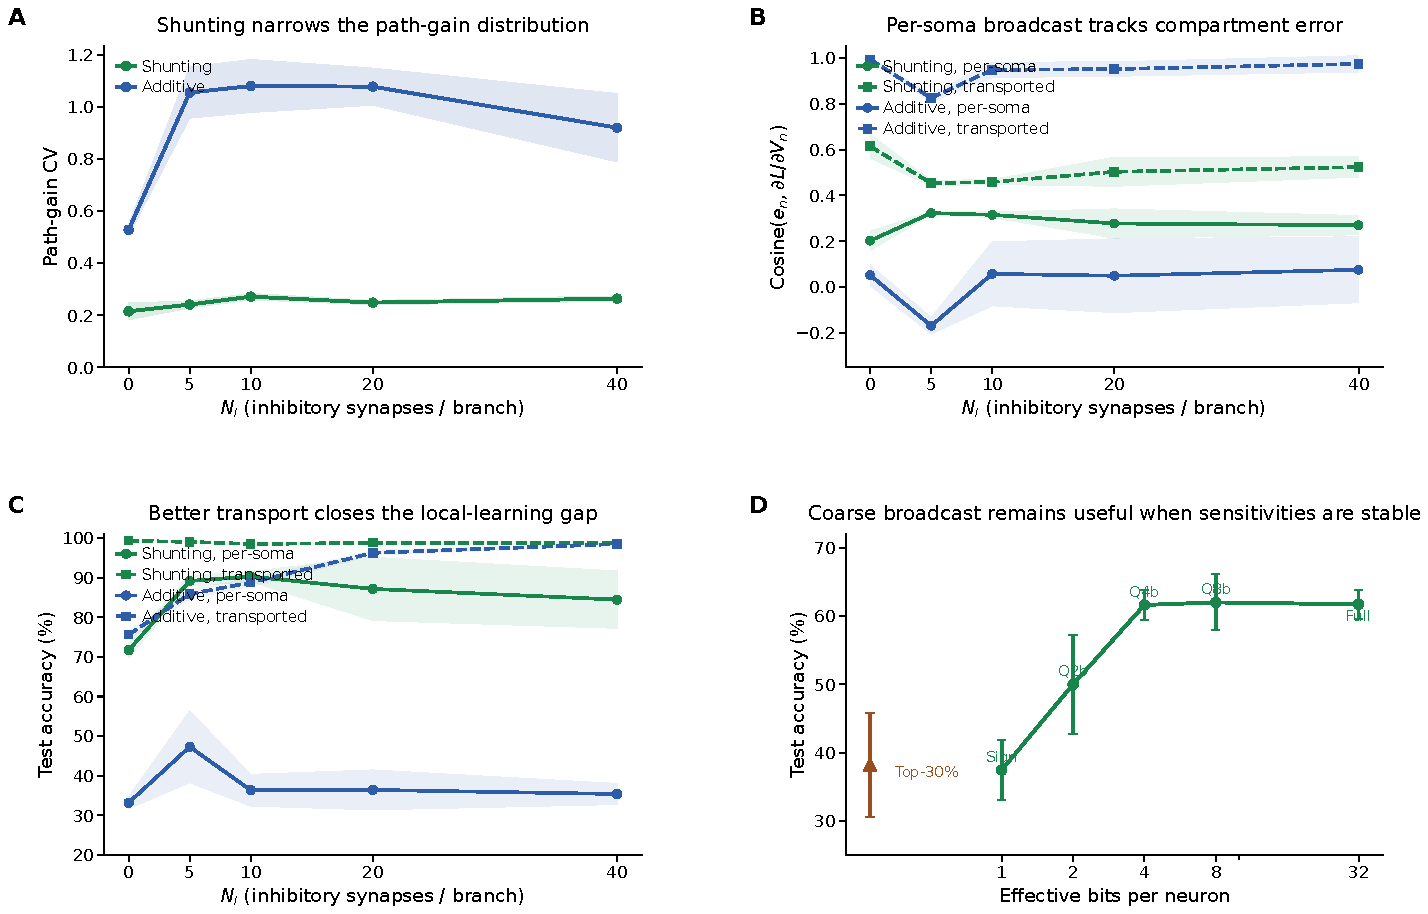
\includegraphics[width=\textwidth]{fig5_mechanistic_evidence.pdf}
\caption{\textbf{Mechanistic chain from path gains to learning.}
\textbf{(A)}~Dendritic path-gain fields at matched inhibition.
\textbf{(B)}~Exact-error compressibility on MNIST: lower rank-$1$ residual and participation rank favor scalar broadcast.
\textbf{(C)}~Post-training inhibitory-conductance interventions (L: learned; 0/sh/m/u: zero, shuffled, mean-clamped, uniform matched).
\textbf{(D)}~Compartment-error fidelity on noise resilience; dashed lines show the transported-error oracle.
\textbf{(E)}~Transported-error learning recovers near-ceiling local learning where rank-$1$ broadcast fails. Error bars denote $\pm$1 s.d.\ across seeds.}
\label{fig:mechanistic}
\end{figure}

\begin{figure}[!t]
\centering
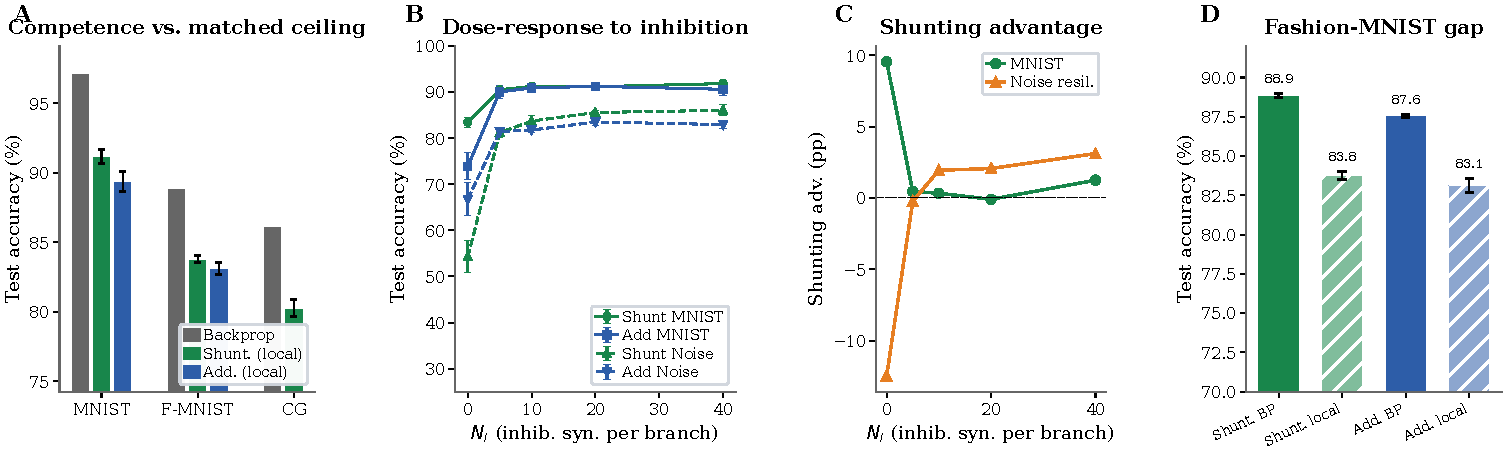
\includegraphics[width=\textwidth]{fig2_competence_regime.pdf}
\caption{\textbf{Capacity-calibrated competence and regime dependence.}
\textbf{(A)}~Matched backprop reference performance vs.\ rank-$1$ 5F LocalCA on MNIST, Fashion-MNIST, and context gating.
\textbf{(B)}~Inhibitory dose-response.
\textbf{(C)}~Morphology-dependent shunting advantage on noise resilience from a 3-seed sweep.
\textbf{(D)}~Additive normalization improves additive LocalCA but remains below the shunting reference. Error bars denote $\pm$1 s.d.\ where available.}
\label{fig:competence_regime}
\end{figure}

\subsection{Setup}

The experiments test five linked predictions: exact factorization should reconstruct autograd gradients; shunting should improve LocalCA direction and scale relative to backpropagation; exact compartment errors should be more compressible under shunting than under matched additive controls; learned inhibition should carry sample-specific pathway structure rather than merely adding conductance load; and replacing the broadcast with transported exact error should largely close the local-learning gap.
We evaluate capacity-calibrated supervised tasks and controlled sweeps that isolate inhibition strength, rule family, broadcast mode, morphology, and architecture.
The main text uses MNIST, Fashion-MNIST \cite{xiao2017fashionmnist}, context gating, noise resilience, and a compressed morphology-regime summary; CIFAR-10 and routed-feedback diagnostics are reported in the appendix (Figs.~\ref{fig:cifar10_mechanism_extension}, \ref{fig:cue_routing}).
Main comparisons are architecture-matched additive vs.\ shunting dendritic cores and local vs.\ backprop training; DFA is a supplementary baseline.
Unless otherwise stated, local runs use 5F with the default neuron-wise broadcast, which reduces to rank-$1$ shared broadcast when hidden width exceeds the decoder-error dimension.
All main-claim dendritic runs use nonnegative conductance transforms and nonnegative first-layer synaptic drive; image inputs are in $[0,1]$, corrupted inputs are clipped back to $[0,1]$, and context gating uses a nonnegative contextual figure-ground MNIST construction.
The transported-error condition is an oracle upper bound derived from Theorem~\ref{thm:tree_backprop}, not the proposed biological rule.
Main mechanistic, oracle, and competence results use $5$ seeds per condition unless noted otherwise.

\subsection{From Exact Factorization to Credit-Signal Fidelity}
\label{sec:grad_fidelity}

To test whether these performance differences correspond to better credit signals, we compare local and backprop gradients on the same batch at the same parameter values.
For each parameter tensor $p$, we compute directional alignment (cosine similarity) and scale mismatch, defined as $|\log_{10}(\|g_p^{\mathrm{local}}\|/\|g_p^{\mathrm{bp}}\|)|$, aggregated by parameter count.

Across the MNIST gradient-dynamics diagnostic, shunting is more aligned with backprop and closer in norm than the additive control at the final checkpoint: weighted cosine rises from $0.005\pm0.026$ to $0.100\pm0.033$, and scale mismatch falls from $0.50\pm0.05$ to $0.26\pm0.05$.
Figure~\ref{fig:gradient_fidelity}A confirms that the implementation matches the theory under the nonnegative-input setup: reconstructing gradients from Corollary~\ref{cor:factorization} using exact compartment errors yields weighted relative reconstruction error below $2\times 10^{-7}$ and weighted scale mismatch below $4\times 10^{-8}$ across runs.
In a few low-norm parameter blocks, cosine becomes numerically unstable even though the reconstruction itself is essentially exact, so we report the norm-based diagnostics in the figure.
Figure~\ref{fig:gradient_fidelity}D shows the same gradient-alignment comparison over training: additive alignment remains near zero at the final checkpoint rather than failing only at one static snapshot. Appendix Fig.~\ref{fig:alignment_norm_dynamics} verifies that the corresponding local and backprop gradient norms remain finite throughout learning, ruling out a trivial zero-gradient explanation.
At the level of the theoretically derived 3F rule, the central non-local approximation is therefore the broadcast substitute for $\partial L/\partial V_n$.

\newpage
\begin{figure}[!t]
\centering
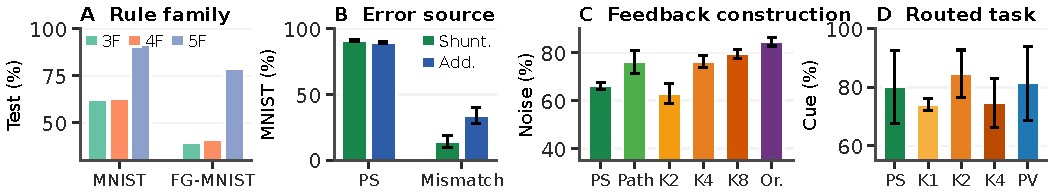
\includegraphics[width=\textwidth]{fig5_rule_feedback_controls.pdf}
\caption{\textbf{Rule and feedback controls.}
\textbf{(A)}~The practical gain comes mainly from the 5F confidence wrapper; 3F/4F remain weak optimizers.
\textbf{(B)}~Replacing the somatic rank-$1$ error with a local-mismatch heuristic collapses learning.
\textbf{(C)}~Richer or transported feedback improves noise resilience. Detailed controls remain in Appendix Fig.~\ref{fig:rule_feedback_design}.}
\label{fig:rule_feedback_controls}
\end{figure}

\subsection{Mechanistic Chain: Path Gains, Broadcast Fidelity, and Oracle Transport}

Figure~\ref{fig:mechanistic} provides the central empirical chain. At matched inhibition ($N_I{=}5$), shunting narrows the MNIST conductance-stage path-gain field (CV $0.23$ vs.\ $1.16$ for additive) and makes the exact compartment-error matrix more compressible: the best rank-$1$ residual drops from $0.83\pm0.07$ to $0.65\pm0.18$, while participation rank drops from $8.5\pm3.3$ to $3.2\pm1.2$. This is the diagnostic matched to the paper's main claim: rank-$1$ broadcast is useful when the exact error field is closer to low rank.

The inhibition intervention shows that the learned inhibitory field is necessary for the trained computation and is not interchangeable with a matched conductance load: zeroing, shuffling, or clamping learned branch inhibition drops MNIST from about $90\%$ to $20$--$26\%$ and noise resilience from about $81\%$ to $10$--$19\%$. The fidelity and oracle panels test the same bottleneck: rank-$1$ broadcast tracks the exact compartment error better under shunting once inhibition is present, transported error reaches about $0.95$--$1.0$ fidelity, and transported learning lifts both cores to $92$--$95\%$ on noise resilience. CIFAR-10 and direct-I versus explicit-I path-gain probes remain appendix diagnostics (Fig.~\ref{fig:cifar10_mechanism_extension}; Table~\ref{tab:input_mode_probe}).

\subsection{Capacity-Calibrated Competence}

In the capacity-calibrated regime, shunting LocalCA remains within about $5$--$6$ percentage points of matched backpropagation on MNIST, Fashion-MNIST, and context gating (Table~\ref{tab:gap_closing}; Fig.~\ref{fig:competence_regime}). Figure~\ref{fig:competence_regime}D shows that additive normalization improves additive LocalCA but remains below the shunting reference, so the gain is not explained by generic voltage normalization alone. Figure~\ref{fig:rule_feedback_controls} summarizes the rule and feedback controls: 5F is the strongest practical optimizer, somatic rank-$1$ error is essential, and higher feedback bandwidth improves the noise-resilience diagnostic.

\subsection{Regime Dependence of the Shunting Advantage}

With matched rank-$1$ broadcast, shunting is modestly better on MNIST, Fashion-MNIST, and context gating, including $0.803\pm0.006$ vs.\ $0.787\pm0.007$ for additive on context gating. The gap grows on inhibition-sensitive noise resilience once inhibitory conductance is present (Fig.~\ref{fig:competence_regime}B). Morphology shifts the useful inhibitory operating regime: different tree depths and branch factors peak at different $N_I$, and the shunting advantage is not monotonic in inhibition (Fig.~\ref{fig:competence_regime}C). Appendix Fig.~\ref{fig:additional_stress_tests} extends this boundary check to depth scaling and noisy error broadcasts.

\section{Discussion and Limitations}
\label{sec:discussion}
We studied local credit assignment in dendritic networks that explicitly represent three biological ingredients often abstracted away in standard neural networks: E/I conductance synapses, shunting inhibition, and tree-structured dendritic branching. The exact gradient derivation shows that these ingredients create a simple decomposition. The synapse-local part of the gradient is available from presynaptic activity, driving force, and input resistance; the only non-local quantity is a compartment-specific error.

The experiments support a coherent mechanism. Branching creates multiple credit paths from distal synapses to the soma, E/I synapse banks set the conductance state of each compartment, and shunting inhibition modulates input resistance along those paths. In the regimes studied here, this makes the exact error field more compressible for rank-$1$ broadcast, improves local-backprop gradient alignment, and reduces scale mismatch. Transported-error oracle experiments show that replacing the broadcast with the exact path-gain-transported error largely closes the local-learning gap, while inhibition interventions show that learned inhibitory conductance carries sample-specific pathway structure rather than merely setting a global conductance scale.

The mechanism has clear limits. Shunting is not a universal substitute for backpropagation, and more inhibition is not always better. The practical 5F rule is an empirical stabilizer rather than a theorem-derived necessity; Eq.~\eqref{eq:compression_condition} is interpretive; activation shape changes the operating regime; and routed or harder-data settings require higher-rank or pathway-specific feedback when the exact error field is not rank-$1$ compressible. The main model uses input-driven shunting inhibition rather than recurrent lateral inhibition, so recurrent inhibitory circuits remain a future direction. The main message is that biophysical dendritic mechanisms can change not only neural representations, but also the geometry of credit assignment.

%=============================================================================
% REFERENCES
%=============================================================================

\begin{thebibliography}{99}

\bibitem{koch1999biophysics}
Koch, C. (1999).
\emph{Biophysics of Computation}.
Oxford University Press.

\bibitem{dayan2001theoretical}
Dayan, P., \& Abbott, L. F. (2001).
\emph{Theoretical Neuroscience}.
MIT Press.

\bibitem{poiarazi2003pyramidal}
Poirazi, P., Brannon, T., \& Mel, B. W. (2003).
Pyramidal neuron as two-layer neural network.
\emph{Neuron}, 37(6), 989--999.

\bibitem{london2005dendritic}
London, M., \& H{\"a}usser, M. (2005).
Dendritic computation.
\emph{Annual Review of Neuroscience}, 28, 503--532.

\bibitem{urbanczik2014dendritic}
Urbanczik, R., \& Senn, W. (2014).
Learning by the dendritic prediction of somatic spiking.
\emph{Neuron}, 81(3), 521--528.

\bibitem{carandini2012normalization}
Carandini, M., \& Heeger, D. J. (2012).
Normalization as a canonical neural computation.
\emph{Nature Reviews Neuroscience}, 13(1), 51--62.

\bibitem{holt1997shunting}
Holt, G. R., \& Koch, C. (1997).
Shunting inhibition does not have a divisive effect on firing rates.
\emph{Neural Computation}, 9(5), 1001--1013.

\bibitem{vogels2011inhibitory}
Vogels, T. P., Sprekeler, H., Zenke, F., Clopath, C., \& Gerstner, W. (2011).
Inhibitory plasticity balances excitation and inhibition in sensory pathways and memory networks.
\emph{Science}, 334(6062), 1569--1573.

\bibitem{lillicrap2016random}
Lillicrap, T. P., Cownden, D., Tweed, D. B., \& Akerman, C. J. (2016).
Random synaptic feedback weights support error backpropagation for deep learning.
\emph{Nature Communications}, 7, 13276.

\bibitem{nokland2016dfa}
N{\o}kland, A. (2016).
Direct feedback alignment provides learning in deep neural networks.
\emph{NeurIPS}, 29.

\bibitem{guerguiev2017segregated}
Guerguiev, J., Lillicrap, T. P., \& Richards, B. A. (2017).
Towards deep learning with segregated dendrites.
\emph{eLife}, 6, e22901.

\bibitem{sacramento2018dendritic}
Sacramento, J., Costa, R. P., Bengio, Y., \& Senn, W. (2018).
Dendritic cortical microcircuits approximate the backpropagation algorithm.
\emph{NeurIPS}, 31.

\bibitem{whittington2019theories}
Whittington, J. C., \& Bogacz, R. (2019).
Theories of error back-propagation in the brain.
\emph{Trends in Cognitive Sciences}, 23(3), 235--250.

\bibitem{richards2019dendritic}
Richards, B. A., \& Lillicrap, T. P. (2019).
Dendritic solutions to the credit assignment problem.
\emph{Current Opinion in Neurobiology}, 54, 28--36.

\bibitem{scellier2017equilibrium}
Scellier, B., \& Bengio, Y. (2017).
Equilibrium propagation.
\emph{Frontiers in Computational Neuroscience}, 11, 24.

\bibitem{song2024prospective}
Song, Y., Millidge, B., Salvatori, T., Lukasiewicz, T., Xu, Z., \& Bogacz, R. (2024).
Inferring neural activity before plasticity as a foundation for learning beyond backpropagation.
\emph{Nature Neuroscience}, 27, 348--358.

\bibitem{gretton2005hsic}
Gretton, A., Bousquet, O., Smola, A. J., \& Sch{\"o}lkopf, B. (2005).
Measuring statistical dependence with Hilbert-Schmidt norms.
\emph{Algorithmic Learning Theory}, 63--77.

\bibitem{fremaux2016three}
Fr{\'e}maux, N., \& Gerstner, W. (2016).
Neuromodulated spike-timing-dependent plasticity, and theory of three-factor learning rules.
\emph{Frontiers in Neural Circuits}, 9, 85.

\bibitem{bellec2020eprop}
Bellec, G., et al. (2020).
A solution to the learning dilemma for recurrent networks of spiking neurons.
\emph{Nature Communications}, 11, 3625.

\bibitem{welford1962note}
Welford, B. P. (1962).
Note on a method for calculating corrected sums of squares and products.
\emph{Technometrics}, 4(3), 419--420.

\bibitem{turrigiano2008homeostatic}
Turrigiano, G. G. (2008).
The self-tuning neuron: synaptic scaling of excitatory synapses.
\emph{Cell}, 135(3), 422--435.

\bibitem{payeur2021burst}
Payeur, A., Guerguiev, J., Zenke, F., Richards, B. A., \& Naud, R. (2021).
Burst-dependent synaptic plasticity can coordinate learning in hierarchical circuits.
\emph{Nature Neuroscience}, 24(7), 1010--1019.

\bibitem{greedy2022burstccn}
Greedy, W., Zhu, H. W., Pemberton, J., Mellor, J., \& Ponte Costa, R. (2022).
Single-phase deep learning in cortico-cortical networks.
\emph{NeurIPS}, 35, 24213--24225.

\bibitem{haider2021latent}
Haider, P., Ellenberger, B., Kriener, L., Jordan, J., Senn, W., \& Petrovici, M. A. (2021).
Latent Equilibrium: A unified learning theory for arbitrarily fast computation with arbitrarily slow neurons.
\emph{NeurIPS}, 34.

\bibitem{hinton2022forward}
Hinton, G. (2022).
The forward-forward algorithm.
\emph{arXiv:2212.13345}.

\bibitem{dellaferrera2022pepita}
Dellaferrera, G., \& Kreiman, G. (2022).
Error-driven input modulation: Solving the credit assignment problem without a backward pass.
\emph{Proceedings of the 39th International Conference on Machine Learning}, \emph{Proceedings of Machine Learning Research}, 162, 4937--4955.

\bibitem{lee2015dtp}
Lee, D.-H., et al. (2015).
Difference target propagation.
\emph{ECML}, 498--515.

\bibitem{meulemans2021dfc}
Meulemans, A., et al. (2021).
Credit assignment in neural networks through deep feedback control.
\emph{NeurIPS}, 34.

\bibitem{millidge2022predictive}
Millidge, B., Seth, A. K., \& Buckley, C. L. (2021).
Predictive coding: A theoretical and experimental review.
\emph{arXiv:2107.12979}.

\bibitem{koch1983nonlinear}
Koch, C., Poggio, T., \& Torre, V. (1983).
Nonlinear interactions in a dendritic tree.
\emph{PNAS}, 80(9), 2799--2802.

\bibitem{silver2010neuronal}
Silver, R. A. (2010).
Neuronal arithmetic.
\emph{Nature Reviews Neuroscience}, 11(7), 474--489.

\bibitem{pal2024local}
Max, K., Kriener, L., Pineda Garc{\'\i}a, G. et al. (2024).
Learning efficient backprojections across cortical hierarchies in real time.
\emph{Nature Machine Intelligence}, 6(6), 619--630.

\bibitem{ma2024auglocal}
Ma, C., Wu, J., Si, C., \& Tan, K. C. (2024).
Scaling supervised local learning with augmented auxiliary networks.
\emph{International Conference on Learning Representations (ICLR)}.

\bibitem{lv2025dll}
Lv, C., Xu, J., Lu, Y., Wang, X., Wang, Z., Xu, Z., Yu, D., Du, X., Zheng, X., \& Huang, X. (2025).
Dendritic Localized Learning: Toward Biologically Plausible Algorithm.
\emph{Proceedings of the 42nd International Conference on Machine Learning}, \emph{Proceedings of Machine Learning Research}, 267, 41682--41700.

\bibitem{erdogan2025ebd}
Erdogan, M., Pehlevan, C., \& Erdogan, A. T. (2025).
Error broadcast and decorrelation as a potential artificial and natural learning mechanism.
\emph{OpenReview}, NeurIPS 2025 spotlight.

\bibitem{kao2024ccl}
Kao, C.-H., \& Hariharan, B. (2024).
Counter-Current Learning: A Biologically Plausible Dual Network Approach for Deep Learning.
\emph{Advances in Neural Information Processing Systems}, 37.

\bibitem{xiao2017fashionmnist}
Xiao, H., Rasul, K., \& Vollgraf, R. (2017).
Fashion-MNIST: A novel image dataset for benchmarking machine learning algorithms.
\emph{arXiv:1708.07747}.

\bibitem{song2005lognormal}
Song, S., Sj{\"o}str{\"o}m, P. J., Reigl, M., Nelson, S., \& Chklovskii, D. B. (2005).
Highly nonrandom features of synaptic connectivity in local cortical circuits.
\emph{PLoS Biology}, 3(3), e68.

\bibitem{buzsaki2014logdynamic}
Buzs{\'a}ki, G., \& Mizuseki, K. (2014).
The log-dynamic brain: How skewed distributions affect network operations.
\emph{Nature Reviews Neuroscience}, 15(4), 264--278.

\bibitem{microns2021functional}
The MICrONS Consortium (2025).
Functional connectomics spanning multiple areas of mouse visual cortex.
\emph{Nature}, 640(8058), 435--447.

\bibitem{loewenstein2011multiplicative}
Loewenstein, Y., Kuras, A., \& Rumpel, S. (2011).
Multiplicative Dynamics Underlie the Emergence of the Log-Normal Distribution of Spine Sizes in the Neocortex In Vivo.
\emph{Journal of Neuroscience}, 31(26), 9481--9488.

\bibitem{megias2001total}
Meg{\'i}as, M., et al. (2001).
Total number and distribution of inhibitory and excitatory synapses on hippocampal CA1 pyramidal cells.
\emph{Neuroscience}, 102(3), 527--540.

\bibitem{nature2026vectorized}
Francioni, V., Tang, V. D., Toloza, E. H. S. et al. (2026).
Vectorized instructive signals in cortical dendrites.
\emph{Nature}. https://doi.org/10.1038/s41586-026-10190-7

\bibitem{iyer2022activedendrites}
Iyer, A., Grewal, K., Velu, A., Souza, L. O., Forest, J., \& Ahmad, S. (2022).
Avoiding catastrophe: Active dendrites enable multi-task learning in dynamic environments.
\emph{Frontiers in Neurorobotics}, 16, 846219.

\end{thebibliography}

%=============================================================================
\clearpage
\appendix
\renewcommand{\thefigure}{S\arabic{figure}}
\setcounter{figure}{0}
\renewcommand{\thetable}{S\arabic{table}}
\setcounter{table}{0}
%=============================================================================

\section{Supplementary Results}
\label{app:extra_results}

\paragraph{Appendix overview.}
The appendix is organized by how directly each result supports the main mechanism. The first block collects rule and feedback controls that complement Fig.~\ref{fig:rule_feedback_controls}. The second block reports competence checks, gradient dynamics, stress tests, and baseline comparisons. The third block contains harder-data, morphology, inhibition, and pathway-feedback diagnostics. The final blocks give implementation, theory, task, and concise secondary weight statistics. Exploratory screens and development summaries that do not directly support a paper claim are omitted.

\paragraph{Boundary diagnostics.}
Several controls are intentionally negative or mixed. The log-gain covariance margin from Eq.~\eqref{eq:compression_condition} is not a positive main result, Double-CIFAR remains near chance even under matched backpropagation, positive cue-routing controls saturate too strongly to separate mechanisms, and the current pathway-vector implementation does not beat the best unstructured low-rank cue-routing control. We include these results to delimit the claim rather than to smooth over failure modes.

\subsection*{Mechanistic Support and Broadcast Controls}

\begin{figure*}[!htbp]
\centering
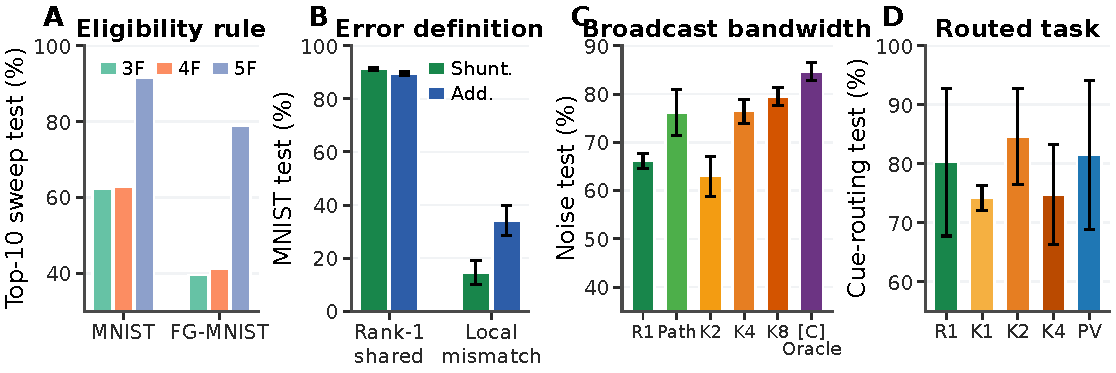
\includegraphics[width=\textwidth]{fig4_rule_feedback_design.pdf}
\caption{\textbf{Local-rule and feedback-design axes.}
\textbf{(A)}~The theoretically derived 3F update and the 4F attenuation proxy are weak practical optimizers in the completed local-competence sweeps; 5F is the strongest empirical wrapper.
\textbf{(B)}~The broadcast definition matters: on MNIST, rank-$1$ shared somatic error is strong, while a local-mismatch error surrogate fails.
\textbf{(C)}~On noise resilience, recursively propagating or increasing the rank of the error field closes much of the gap between rank-$1$ broadcast and exact path transport.
\textbf{(D)}~Cue routing probes a branch-specific regime: higher rank helps, while the current pathway-vector implementation is useful but not yet better than the best unstructured low-rank control. Error bars denote $\pm$1 s.d.\ where five-seed summaries are available.}
\label{fig:rule_feedback_design}
\end{figure*}

\subsection*{Rule-Family Ranking}

\begin{table}[!htbp]
\centering
\small
\begin{tabular}{@{}llcc@{}}
\toprule
\textbf{Dataset} & \textbf{Rule} & \textbf{Top-10 valid} & \textbf{Top-10 test} \\
\midrule
MNIST & 3F & 0.611 & 0.622 \\
MNIST & 4F & 0.620 & 0.628 \\
MNIST & 5F & \textbf{0.912} & \textbf{0.916} \\
\midrule
Context gating & 3F & 0.398 & 0.396 \\
Context gating & 4F & 0.411 & 0.411 \\
Context gating & 5F & \textbf{0.807} & \textbf{0.789} \\
\bottomrule
\end{tabular}
\caption{\textbf{Rule-family ranking.} Top-10 mean across completed local-competence sweeps.}
\label{tab:variant_ranking}
\end{table}

\subsection*{Competence, Verification, and Stress Tests}

\subsection*{Local Competence and Regime Dependence}

\begin{table}[t]
\centering
\small
\begin{tabular}{@{}lcccc@{}}
\toprule
\textbf{Dataset} & \textbf{BP ceiling} & \textbf{Shunting local} & \textbf{Additive local} & \textbf{BP gap} \\
\midrule
MNIST & 0.971 & $0.912\pm0.005$ & $0.894\pm0.007$ & 5.9\% \\
Fashion-MNIST & 0.889 & $0.838\pm0.003$ & $0.831\pm0.004$ & 5.1\% \\
Context gating & 0.861 & $0.803\pm0.006$ & $0.787\pm0.007$ & 5.8\% \\
\bottomrule
\end{tabular}
\caption{\textbf{Local competence.} Backprop ceilings are matched-capacity shunting references from dedicated $5$-seed standard-training refreshes for MNIST and context gating and from the dedicated $5$-seed Fashion-MNIST competence sweep. Local values are 5F with rank-$1$ broadcast and local decoder updates. Context gating additionally uses an HSIC auxiliary objective (weight $0.01$; Appendix~\ref{app:hsic}). Error bars on local values: $\pm$1 s.d.\ across 5 seeds.}
\label{tab:gap_closing}
\end{table}


\subsection*{Extended Gradient Analysis and $N_I$ Sweep Detail}

\begin{figure*}[t]
\centering
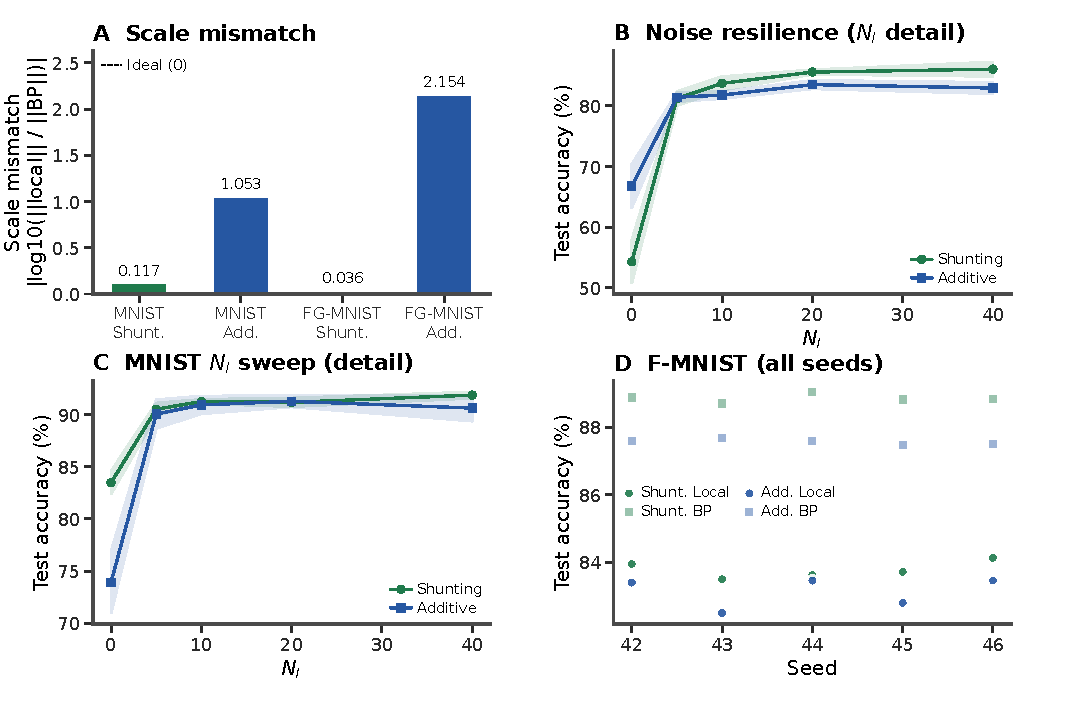
\includegraphics[width=0.95\textwidth]{fig_s2_gradient_extended.pdf}
\caption{\textbf{Extended gradient and $N_I$ analysis (supplementary).} \textbf{(A)}~Scale mismatch bars from a separate matched-weight static diagnostic; these values should not be compared directly to the checkpointed final-state diagnostic in Fig.~\ref{fig:gradient_fidelity}. Shunting achieves near-ideal scale ($0.117$); additive exhibits order-of-magnitude distortion ($>1.0$). \textbf{(B)}~Noise-resilience $N_I$ dose-response with error bands ($\pm$1 s.d.). \textbf{(C)}~MNIST $N_I$ dose-response detail with error bands. \textbf{(D)}~Fashion-MNIST individual seeds for all conditions, showing consistency across runs.}
\end{figure*}

\paragraph{Alignment dynamics are not a zero-gradient artifact.}
To check whether low additive alignment could be caused by vanishing gradients, we analyzed a separate 3-seed checkpoint trajectory with parameter-level LocalCA and backprop gradients. The additive local gradients are nonzero throughout training (weighted norm range $9.5{\times}10^{-4}$--$9.5{\times}10^{-3}$), and the corresponding backprop gradients are also nonzero ($2.3{\times}10^{-5}$--$5.7{\times}10^{-3}$). The low additive cosine therefore reflects directional and scale mismatch, not absent gradients: additive 5F cosine stays near zero from epoch $0$ to epoch $50$ ($0.018$ to $0.005$), while its local/backprop norm ratio falls from about $8.8{\times}10^2$ to $0.69$.

\begin{figure}[t]
\centering
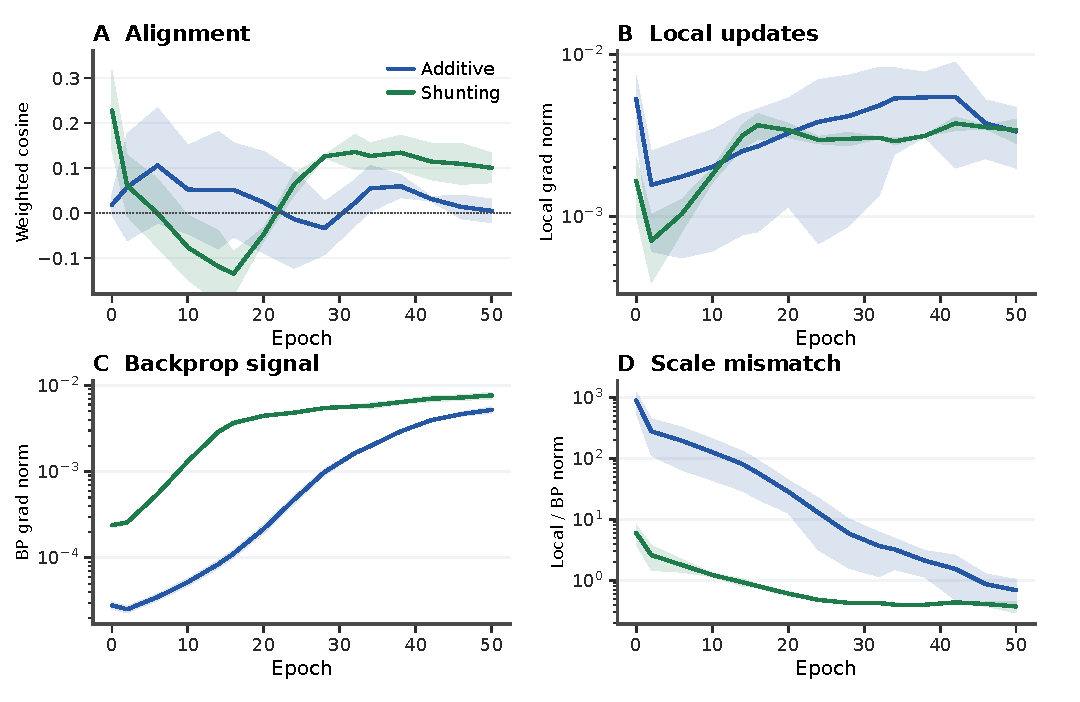
\includegraphics[width=0.98\textwidth]{fig_s_alignment_norm_dynamics.pdf}
\caption{\textbf{Alignment dynamics with explicit gradient-norm checks.}
\textbf{(A)} Weighted LocalCA-vs.-backprop cosine over training for the 5F rule. \textbf{(B,C)} Weighted local and backprop gradient norms stay nonzero for both additive and shunting models. \textbf{(D)} The additive control begins with a much larger scale mismatch, then approaches the backprop scale without recovering strong directional alignment. Shading is s.d.\ across 3 seeds.}
\label{fig:alignment_norm_dynamics}
\end{figure}

\subsection*{Verification and Reproducibility}

\begin{figure*}[t]
\centering
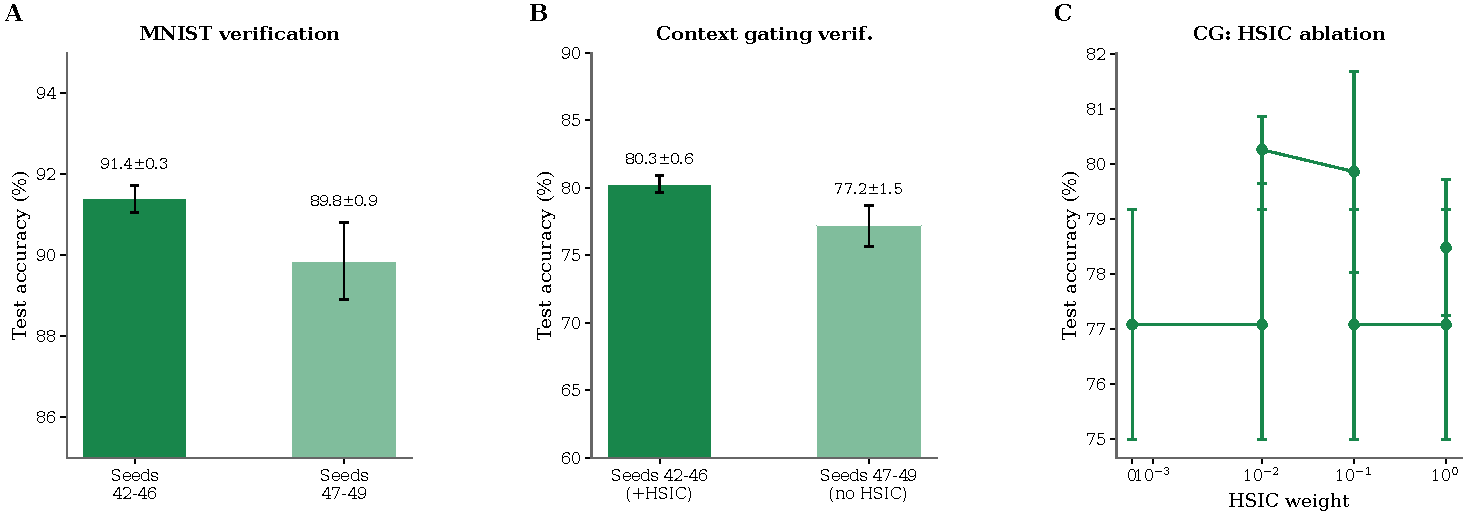
\includegraphics[width=0.95\textwidth]{fig_s4_verification.pdf}
\caption{\textbf{Verification and reproducibility (supplementary).} \textbf{(A)}~MNIST verification: main seeds (42--46) yield $91.4\pm0.3$\%; held-out seeds (47--49) yield $89.8\pm0.9$\%, confirming generalization. \textbf{(B)}~Context gating verification: main seeds ($+$HSIC) $80.3\pm0.6$\%; held-out seeds (no HSIC) $77.2\pm1.5$\%. The roughly $3$~pp gap reflects HSIC removal, not seed sensitivity. \textbf{(C)}~HSIC weight ablation on context gating: moderate weights ($0.01$--$0.1$) perform best.}
\label{fig:verification_appendix}
\end{figure*}

\subsection*{Additional Stress Tests}

\begin{figure*}[t]
\centering
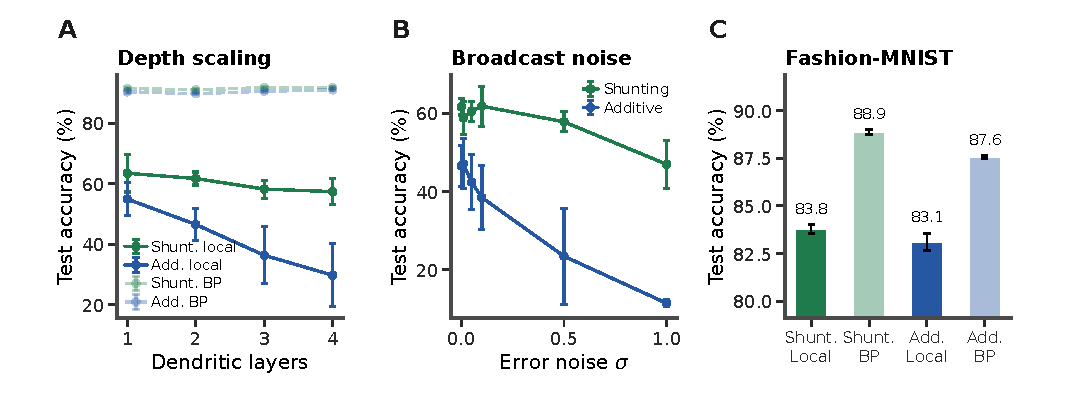
\includegraphics[width=0.95\textwidth]{fig_additional_stress_tests.pdf}
\caption{\textbf{Additional stress tests.} \textbf{(A)}~Depth scaling: shunting local (green) degrades more gracefully from 63.5\% to 57.4\%; additive local (blue) drops from 54.9\% to 29.7\%. Backprop ceilings (dashed) remain stable. \textbf{(B)}~Broadcast-noise robustness: shunting remains stable for $\sigma\!\leq\!0.1$; additive degrades rapidly and reaches chance at $\sigma\!=\!1$. \textbf{(C)}~Fashion-MNIST: the shunting gain is modest on this cleaner benchmark (83.8\% local vs.\ 88.9\% backprop), consistent with the regime-dependent story in the main text.}
\label{fig:additional_stress_tests}
\end{figure*}

\subsection*{FA/DFA Baseline Comparison}

\begin{figure*}[t]
\centering
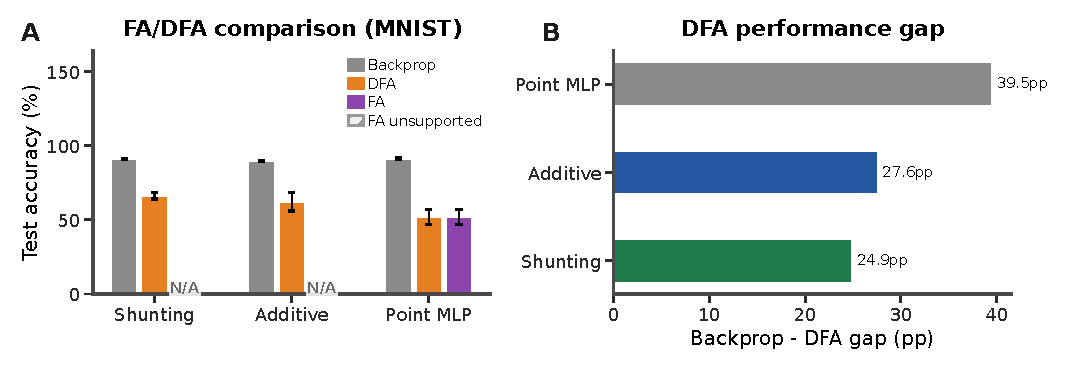
\includegraphics[width=0.95\textwidth]{fig_s5_fa_dfa.pdf}
\caption{\textbf{Feedback alignment baselines (MNIST).} \textbf{(A)}~Grouped comparison: standard backprop (neutral gray), DFA (orange), and FA (purple). Hatched N/A markers indicate that FA is not implemented for the block-structured dendritic architectures because the random feedback matrices are not dimensionally compatible with the tree-structured branch updates. DFA achieves 66.1\% on shunting vs.\ 62.2\% additive vs.\ 51.8\% point MLP. \textbf{(B)}~Backprop$-$DFA gap: dendritic architectures (24.9--27.6~pp) show smaller gaps than point MLPs (39.5~pp), suggesting conductance-based architecture is partially compatible with random feedback.}
\label{fig:fa_dfa_appendix}
\end{figure*}

\subsection*{CIFAR-10 Results}

\begin{figure*}[t]
\centering
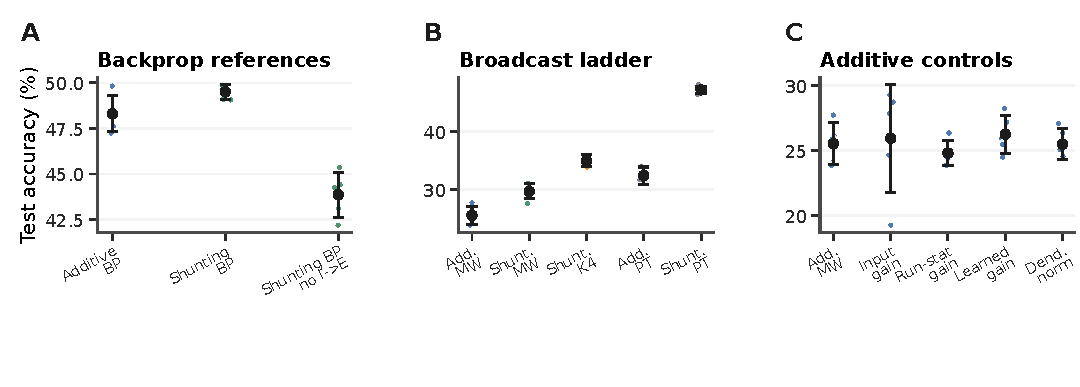
\includegraphics[width=0.98\textwidth]{fig_s_cifar10_control_ladder_20260427.pdf}
\caption{\textbf{CIFAR-10 control ladder in the compact direct-I-stream family.}
\textbf{(A)}~Matched backprop ceilings. With nonnegative inputs and a nonlinear decoder, shunting slightly exceeds additive under standard training, and removing learned I-to-E conductance lowers the shunting ceiling.
\textbf{(B)}~Broadcast ladder. Rank-$1$ broadcast remains weak on this harder dataset, rank-$4$ improves partially, and exact transported error nearly reaches the shunting backprop ceiling.
\textbf{(C)}~Additive fairness controls. Input-dependent gain, running-stat gain, learned gain, and dendritic normalization do not rescue additive rank-$1$ broadcast. This figure is a harder-data diagnostic, not a claim of competitive CIFAR-10 benchmarking.}
\label{fig:cifar10_mechanism_extension}
\end{figure*}

\begin{table*}[t]
\centering
\scriptsize
\renewcommand{\arraystretch}{1.06}
\setlength{\tabcolsep}{3pt}
\begin{tabular}{@{}L{0.32\linewidth}L{0.12\linewidth}L{0.24\linewidth}L{0.10\linewidth}L{0.12\linewidth}@{}}
\toprule
\textbf{Condition} & \textbf{Core} & \textbf{Training / broadcast} & \textbf{I-to-E} & \textbf{Test acc.} \\
\midrule
standard & additive & backprop & yes & $48.3 \pm 1.0$ \\
standard & shunting & backprop & yes & $\mathbf{49.5 \pm 0.4}$ \\
standard, no learned inhibition & shunting & backprop & no & $43.9 \pm 1.2$ \\
\midrule
rank-$1$ & additive & 5F per-soma & yes & $25.5 \pm 1.6$ \\
rank-$1$, input-dependent gain & additive & 5F per-soma & yes & $25.9 \pm 4.1$ \\
rank-$1$, running-stat gain & additive & 5F per-soma & yes & $24.8 \pm 0.9$ \\
rank-$1$, learned gain & additive & 5F per-soma & yes & $26.3 \pm 1.5$ \\
rank-$1$, dendritic normalization & additive & 5F per-soma & yes & $25.5 \pm 1.2$ \\
rank-$1$ & shunting & 5F per-soma & yes & $29.7 \pm 1.3$ \\
rank-$1$, no learned inhibition & shunting & 5F per-soma & no & $22.3 \pm 0.7$ \\
\midrule
transported error & additive & 5F path transport & yes & $32.4 \pm 1.5$ \\
rank-$4$ & shunting & 5F low-rank & yes & $35.0 \pm 1.0$ \\
transported error & shunting & 5F path transport & yes & $\mathbf{47.2 \pm 0.6}$ \\
transported error, no learned inhibition & shunting & 5F path transport & no & $38.6 \pm 1.0$ \\
\bottomrule
\end{tabular}
\renewcommand{\arraystretch}{1.0}
\caption{\textbf{Exact CIFAR-10 values for the 70-run control ladder (5 seeds per condition, validation-best epoch).} All rows use flattened CIFAR-10 in $[0,1]$, nonnegative transfer outputs, positive conductance transforms, a compact depth-$4$ dendritic core, and a nonlinear decoder. LocalCA maps output error back to decoder-input/soma coordinates through the decoder Jacobian. The useful conclusions are narrow but important: learned shunting slightly improves the matched backprop ceiling, learned I-to-E conductance is necessary for the strongest shunting results, transported error nearly closes the shunting LocalCA gap, and additive rank-$1$ fairness controls do not explain the transported-shunting result.}
\label{tab:cifar10_mechanism_extension}
\end{table*}

Table~\ref{tab:cifar10_mechanism_extension} provides the exact values for the appendix CIFAR-10 figure. In this stronger compact direct-I-stream family, shunting performs well under standard training ($49.5\%$ vs.\ $48.3\%$ for additive), so the harder-data stress test does not unfairly penalize the shunting architecture. The broadcast-fidelity ladder also survives once decoder-aware soma mapping is used: additive LocalCA reaches $25.5\%$ under rank-$1$ per-soma broadcast and $32.4\%$ under transported error, while shunting rises from $29.7\%$ under rank-$1$ broadcast to $35.0\%$ with random low-rank $K{=}4$ and $47.2\%$ with transported error, nearly matching the $49.5\%$ shunting backprop ceiling. Removing learned I-to-E conductance lowers the shunting ceiling by $5.7$~pp and transported LocalCA by $8.6$~pp, making this the clearest harder-data evidence that inhibitory conductance is part of the useful credit geometry rather than just an added architectural detail.

A routed Double-CIFAR follow-up with strictly nonnegative router outputs was also not included as positive evidence. The task remained near chance even under matched backprop: additive BP reached $10.9\pm0.7\%$, shunting BP with learned I-to-E reached $11.6\pm0.4\%$, and the strongest LocalCA condition, shunting transported error with learned I-to-E, reached only $11.7\pm0.3\%$. We therefore treat this as a failed hard routed-task screen and keep the stronger compact CIFAR-10 control ladder as the paper's harder-data diagnostic.

\subsection*{Additive Normalization Control}

\begin{figure*}[t]
\centering
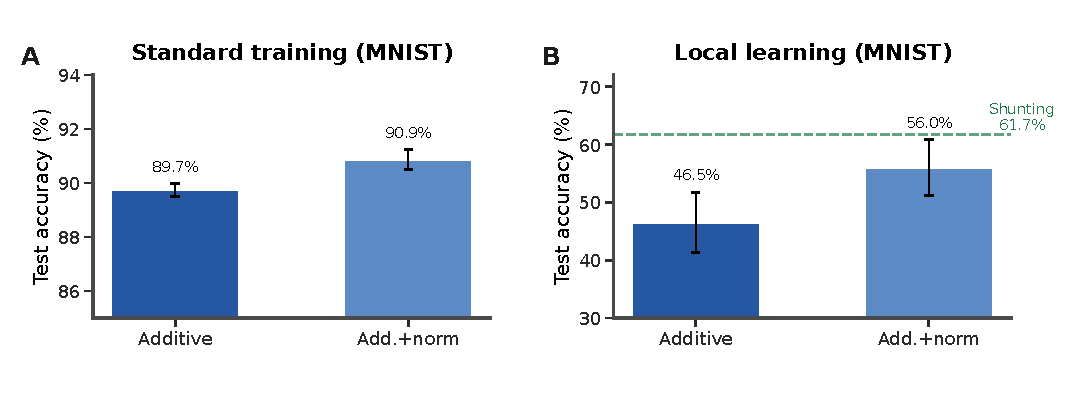
\includegraphics[width=0.95\textwidth]{fig_additive_norm_control.pdf}
\caption{\textbf{Additive + normalization control (MNIST).} \textbf{(A)}~Standard backprop: normalization provides a small boost (89.7\% $\to$ 90.9\%). \textbf{(B)}~Local learning: normalization improves additive from 46.5\% to 56.0\% ($+9.5$~pp), partially closing the gap to shunting (61.7\%, dashed green). The remaining gap ($-5.7$~pp) indicates that shunting provides benefits beyond simple voltage normalization.}
\label{fig:additive_norm_control}
\end{figure*}

\subsection*{Dendritic Morphology, Pathway Structure, and Supportive Extensions}

\subsection*{Morphology $\times$ Inhibition Regime Map}

This supportive regime map tests whether tree geometry changes the inhibitory operating point at which shunting helps. We treat it as evidence that morphology changes the useful inhibition regime; a fuller mechanistic account would still require matched theory diagnostics for each cell in the grid.

\begin{figure*}[t]
\centering
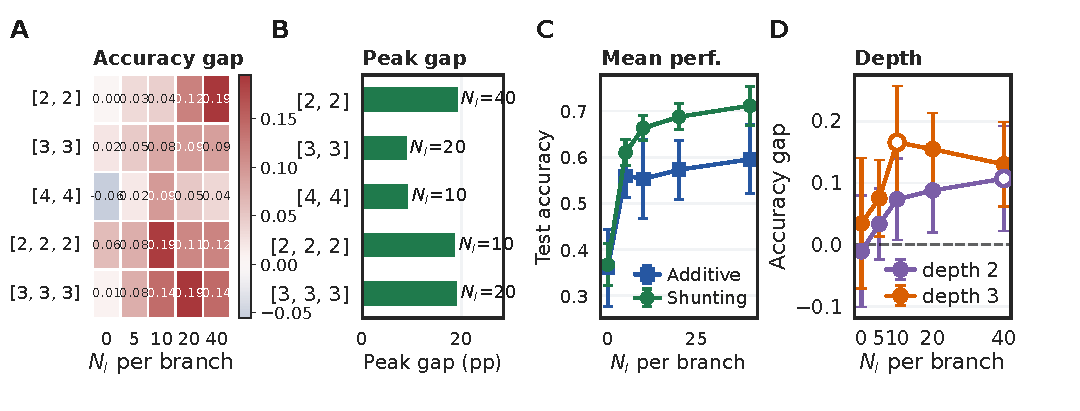
\includegraphics[width=0.98\textwidth]{fig_morphology_ie_regime.pdf}
\caption{\textbf{Morphology shifts the useful inhibitory regime.}
\textbf{(A)}~Shunting-minus-additive LocalCA accuracy gap across dendritic morphologies and inhibitory synapse counts.
\textbf{(B)}~Best inhibitory count for each morphology.
\textbf{(C)}~Representative path-gain diagnostic for selected morphology cells, used to connect the performance map to credit geometry.
\textbf{(D)}~Average shunting advantage by depth, with markers showing the peak inhibitory count for each depth.}
\label{fig:morphology_ie_regime}
\end{figure*}

\subsection*{Input-Mode Probe: Direct Inhibitory Stream vs.\ Explicit Inhibitory Cells}

The main experiments use input-driven inhibitory streams: the transfer layer provides nonnegative excitatory and inhibitory channels from the external input, and excitatory dendrites receive learned I-to-E conductance banks directly. To test whether the same mechanism can be generated by an explicit feedforward inhibitory population, we ran a one-feedforward-layer noise-resilience probe that preserves the relevant dendritic depth ($[3,3]$ morphology). In this clean setting, explicit inhibitory cells reach $94.2\pm0.2\%$ under path-transport LocalCA when their dendrites use the same update policy as excitatory dendrites, $93.8\pm0.2\%$ when those inhibitory-cell updates are frozen, and $95.1\pm0.3\%$ under standard backprop. Direct input-driven inhibition gives the expected broadcast-fidelity ladder on the same one-layer architecture: rank-$1$ broadcast reaches $85.2\pm0.7\%$, while exact path transport reaches $95.2\pm0.0\%$. Thus explicit inhibitory cells can generate useful path-gain structure once the architecture isolates the dendritic-path question. The older two-feedforward-layer explicit-I diagnostic was much weaker (about $58$--$63\%$ under LocalCA despite a $94.7\%$ backprop ceiling), so we treat it as evidence that deeper explicit $E\to I\to E$ graphs need graph-aware local errors, not as evidence against inhibition-mediated path gains.

\begin{table}[t]
\centering
\small
\renewcommand{\arraystretch}{1.08}
\setlength{\tabcolsep}{5pt}
\begin{tabular}{@{}L{0.32\linewidth}L{0.39\linewidth}L{0.18\linewidth}@{}}
\toprule
\textbf{Inhibitory input mode} & \textbf{Training / broadcast} & \textbf{Test accuracy} \\
\midrule
Direct inhibitory stream (\texttt{input\_mode=1}) & LocalCA, per-soma rank-$1$ & $0.852 \pm 0.007$ \\
Direct inhibitory stream (\texttt{input\_mode=1}) & LocalCA, exact path transport & $\mathbf{0.952 \pm 0.000}$ \\
Explicit I cells (\texttt{input\_mode=0}) & LocalCA, path transport, I-cell updates on & $0.942 \pm 0.002$ \\
Explicit I cells (\texttt{input\_mode=0}) & LocalCA, path transport, I-cell updates frozen & $0.938 \pm 0.002$ \\
Explicit I cells (\texttt{input\_mode=0}) & standard backprop & $0.951 \pm 0.003$ \\
\bottomrule
\end{tabular}
\caption{\textbf{One-feedforward-layer input-mode path-gain probe on noise resilience (3 seeds).} All rows use one excitatory dendritic population with $[3,3]$ morphology and nonnegative inputs. The direct-I rows have no explicit inhibitory neurons; the input stream drives learned branch-level inhibitory conductance banks directly. The explicit-I rows use a matched inhibitory population with $[3,3]$ morphology. \texttt{local\_ca} updates explicit inhibitory-cell dendrites with the same policy used for excitatory dendrites, while \texttt{freeze} holds those dendrites fixed but still lets excitatory I-to-E synapses learn. Exact path transport closes the direct-I rank-$1$ gap, and explicit inhibitory cells nearly match both direct-I path transport and the explicit-I backprop ceiling.}
\label{tab:input_mode_probe}
\end{table}

\paragraph{Post-training inhibition intervention and exact-error rank.}
We next tested whether learned inhibitory conductance carries task-specific structure rather than only changing global scale. We replayed trained shunting LocalCA checkpoints while replacing the branch-level inhibitory conductance with four post-training interventions: zero inhibition, sample-shuffled inhibition, per-branch batch means, or one uniform matched mean. On a $512$-example held-out subset, learned MNIST inhibition at $N_I{=}5$ gives $90.4\pm1.1\%$ accuracy, while the four interventions drop to $19.8$--$26.4\%$. On noise resilience at $N_I{=}10$, learned inhibition gives $80.5\pm2.4\%$, while the interventions drop to $10.3$--$19.3\%$. Thus the inhibitory field is not interchangeable with a matched global conductance load. We also computed the SVD of exact compartment-error matrices across samples and compartments. At matched MNIST $N_I{=}5$, shunting has lower rank-$1$ residual than additive ($0.65\pm0.18$ vs.\ $0.83\pm0.07$) and lower participation rank ($3.2\pm1.2$ vs.\ $8.5\pm3.3$), supporting the path-gain compressibility interpretation.

We also computed the direct log-gain covariance margin in Eq.~\eqref{eq:compression_condition} on the selected morphology diagnostic checkpoints. The margin is zero when no inhibitory conductance is present and slightly negative in the inhibited shunting selections ($-2.5\times10^{-3}$, $-5.0\times10^{-4}$, and $-2.8\times10^{-4}$ at $N_I{=}5,20,40$). We therefore do not use this covariance condition as a positive main result. Its role is to clarify when shunting should compress gains; the empirical claim rests on the measured comparative path-gain dispersion, exact-error rank, and inhibition-intervention diagnostics.

\begin{figure}[t]
\centering
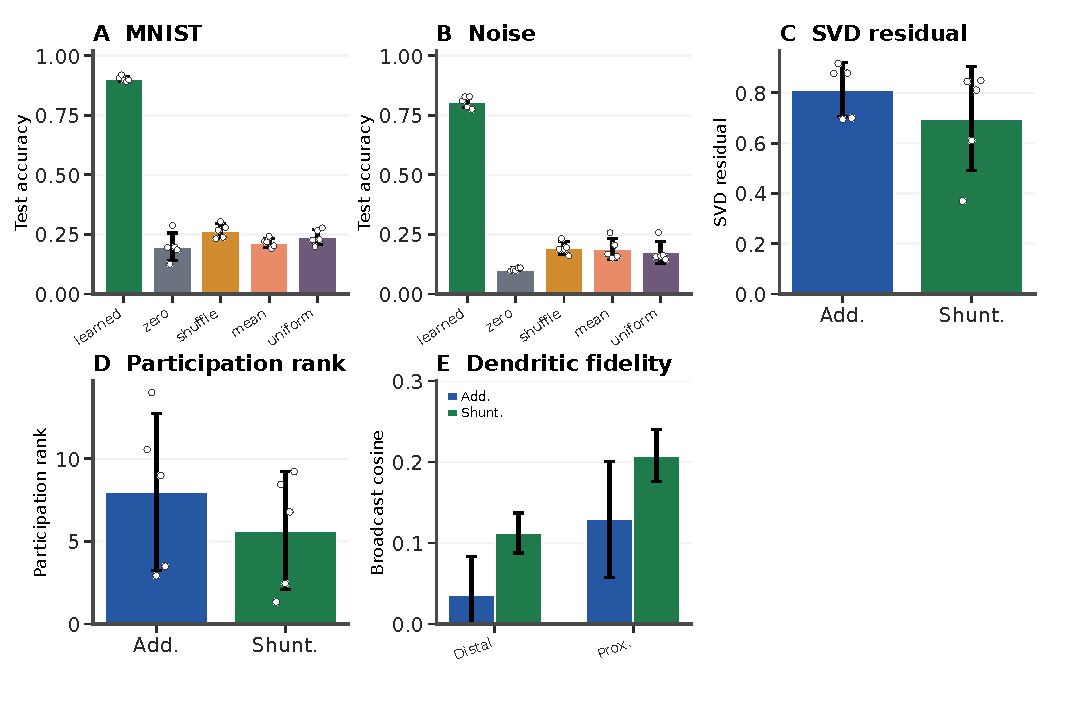
\includegraphics[width=0.98\textwidth]{fig_s_inhibition_causality_error_rank.pdf}
\caption{\textbf{Post-training inhibition intervention and exact-error compressibility.}
\textbf{(A,B)} Post-training inhibitory-conductance interventions on trained shunting LocalCA checkpoints. Accuracy is measured on a $512$-example held-out subset; dots show seeds. Removing, shuffling, or clamping learned inhibition collapses performance, showing that the learned inhibitory field carries sample-specific task structure. \textbf{(C,D)} SVD diagnostics of the exact compartment-error matrix on matched MNIST $N_I{=}5$ runs. Shunting has a smaller rank-$1$ residual and lower participation rank than additive, so the exact error field is more compressible. Error bars are s.d.\ across $5$ seeds.}
\label{fig:inhibition_causality_error_rank}
\end{figure}

\subsection*{Cue-Routing Feedback-Rank Diagnostic}
\label{sec:cue_routing}

Cue routing tests the regime where one shared teaching signal is expected to fail: context determines which noisy cue is reliable, so different pathways should receive different credit. Figure~\ref{fig:cue_routing} shows that the benchmark is learnable and that moving beyond rank-$1$ feedback helps, but the current path-structured variant does not yet beat the best unstructured low-rank setting. We therefore interpret this result as a failure-mode and rank-requirement diagnostic, not as a solved structured-feedback method.

\begin{figure}[t]
\centering
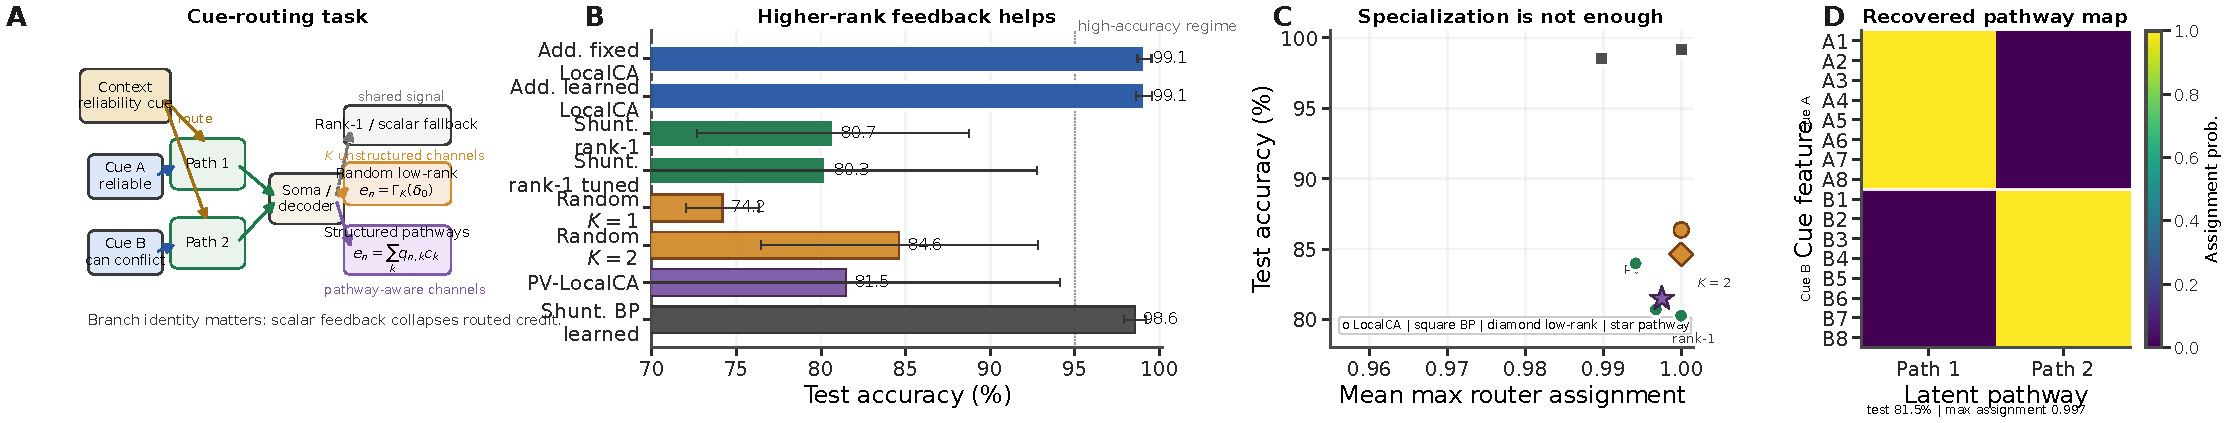
\includegraphics[width=0.95\textwidth]{fig6_cue_routing.pdf}
\caption{\textbf{Structured feedback when rank-$1$ broadcast fails.}
\textbf{(A)}~Cue-routing task schematic. Context determines which noisy cue is reliable on each trial, so different dendritic pathways should receive different teaching signals.
\textbf{(B)}~Five-seed comparison of rank-$1$, random low-rank, and pathway-structured feedback. Moving beyond rank-$1$ helps, while the best structured repair remains open.
\textbf{(C)}~Test accuracy vs.\ router specialization across learned-router conditions. High specialization alone does not guarantee success.
\textbf{(D)}~Recovered pathway assignments for a representative learned-router run. Cue-A and cue-B features segregate into separate latent pathways even when feedback quality, rather than router discreteness, is the limiting factor.}
\label{fig:cue_routing}
\end{figure}

\subsection*{Random Low-Rank Broadcast Channels}

\begin{table}[t]
\centering
\small
\renewcommand{\arraystretch}{1.08}
\setlength{\tabcolsep}{5pt}
\begin{tabular}{@{}lll@{}}
\toprule
\textbf{Setting} & \textbf{Broadcast} & \textbf{Test accuracy} \\
\midrule
\multicolumn{3}{@{}l}{\emph{Noise resilience, shunting, rank bridge}} \\
per-soma & rank-1 per-soma & $0.662 \pm 0.016$ \\
path propagation & recursive attenuation proxy & $0.762 \pm 0.047$ \\
low-rank & $K{=}1$ & $0.453 \pm 0.126$ \\
low-rank & $K{=}2$ & $0.630 \pm 0.042$ \\
low-rank & $K{=}4$ & $0.764 \pm 0.025$ \\
low-rank & $K{=}8$ & $0.795 \pm 0.019$ \\
path transport & exact conductance-stage transport & $\mathbf{0.847 \pm 0.018}$ \\
\addlinespace[2pt]
\multicolumn{3}{@{}l}{\emph{Cue routing, learned shunting router, rank/structure sweep}} \\
per-soma & tuned rank-1 & $0.803 \pm 0.125$ \\
low-rank & $K{=}1$ & $0.742 \pm 0.022$ \\
low-rank & $K{=}2$ & $\mathbf{0.846 \pm 0.082}$ \\
low-rank & $K{=}4$ & $0.748 \pm 0.085$ \\
pathway-vector & tuned structured rank-$2$ & $0.815 \pm 0.126$ \\
\bottomrule
\end{tabular}
\renewcommand{\arraystretch}{1.0}
\caption{\textbf{Rank bridge and rank-structure comparison.} On shunting noise resilience, both the current path-propagation proxy and higher-rank random low-rank broadcast close a substantial fraction of the gap between rank-$1$ per-soma and exact path transport, with low-rank continuing to improve up to $K{=}8$. On cue routing, the learned-router sweep shows that moving beyond rank-$1$ helps, but the best current unstructured low-rank setting ($K{=}2$) is still slightly better than the tuned structured pathway-vector variant. We therefore interpret routed credit assignment as an open higher-rank problem rather than as a solved pathway-vector rescue.}
\label{tab:low_rank_broadcast}
\end{table}


\subsection*{Frozen Activation-Choice Audit}

\begin{table*}[t]
\centering
\small
\renewcommand{\arraystretch}{1.08}
\setlength{\tabcolsep}{5pt}
\begin{tabular}{@{}llccc@{}}
\toprule
\textbf{Dataset / strategy} & \textbf{Core} & \textbf{$N_I$} & \textbf{Identity (\texttt{none})} & \textbf{Frozen \texttt{param\_tanh}} \\
\midrule
MNIST / LocalCA & additive & 0  & $0.780 \pm 0.014$ & $0.709 \pm 0.037$ \\
MNIST / LocalCA & additive & 10 & $0.907 \pm 0.003$ & $0.881 \pm 0.005$ \\
MNIST / LocalCA & shunting & 0  & $0.841 \pm 0.007$ & $0.778 \pm 0.020$ \\
MNIST / LocalCA & shunting & 10 & $0.905 \pm 0.009$ & $0.840 \pm 0.016$ \\
\addlinespace[2pt]
Noise resilience / LocalCA & additive & 0  & $0.590 \pm 0.162$ & $0.109 \pm 0.006$ \\
Noise resilience / LocalCA & additive & 10 & $0.859 \pm 0.001$ & $0.772 \pm 0.009$ \\
Noise resilience / LocalCA & shunting & 0  & $0.411 \pm 0.028$ & $0.331 \pm 0.020$ \\
Noise resilience / LocalCA & shunting & 10 & $0.769 \pm 0.004$ & $0.701 \pm 0.006$ \\
\addlinespace[2pt]
MNIST / backprop & additive & 0  & $0.925 \pm 0.001$ & $0.942 \pm 0.001$ \\
MNIST / backprop & additive & 10 & $0.921 \pm 0.001$ & $0.950 \pm 0.001$ \\
MNIST / backprop & shunting & 0  & $0.963 \pm 0.0004$ & $0.950 \pm 0.001$ \\
MNIST / backprop & shunting & 10 & $0.967 \pm 0.001$ & $0.946 \pm 0.001$ \\
\addlinespace[2pt]
Noise resilience / backprop & additive & 0  & $0.896 \pm 0.003$ & $0.106 \pm 0.007$ \\
Noise resilience / backprop & additive & 10 & $0.893 \pm 0.002$ & $0.927 \pm 0.002$ \\
Noise resilience / backprop & shunting & 0  & $0.898 \pm 0.001$ & $0.869 \pm 0.002$ \\
Noise resilience / backprop & shunting & 10 & $0.926 \pm 0.001$ & $0.912 \pm 0.001$ \\
\bottomrule
\end{tabular}
\renewcommand{\arraystretch}{1.0}
\caption{\textbf{Frozen activation-shape audit on matched dendritic architectures (5 seeds per condition).} Identity (\texttt{none}) and a frozen bounded post-voltage reactivation \texttt{param\_tanh} lead to markedly different operating regimes under nonnegative first-layer synaptic drive. In this audit, identity is the safer LocalCA choice on both MNIST and the noise-resilience task, while the backprop effect is strongly regime-dependent: frozen \texttt{param\_tanh} helps additive most clearly in the inhibited noise-resilience setting ($N_I{=}10$) but collapses it at $N_I{=}0$. These runs match additive reactivation initialization to the shunting setting and hold the activation parameters fixed, isolating activation shape from both additive/shunting initialization differences and activation learning itself.}
\end{table*}

\begin{table*}[t]
\centering
\small
\renewcommand{\arraystretch}{1.08}
\setlength{\tabcolsep}{4.5pt}
\begin{tabular}{@{}llcll@{}}
\toprule
\textbf{Dataset} & \textbf{Core} & \textbf{$N_I$} & \textbf{Identity (\texttt{none})} & \textbf{Frozen \texttt{param\_tanh}} \\
\midrule
MNIST & additive & 0  & CV $0.280$, cosine $0.220$ & CV $1.122$, cosine $0.074$ \\
MNIST & additive & 10 & CV $0.310$, cosine $0.212$ & CV $1.079$, cosine $0.094$ \\
MNIST & shunting & 0  & CV $0.393$, cosine $0.170$ & CV $0.770$, cosine $0.114$ \\
MNIST & shunting & 10 & CV $0.385$, cosine $0.281$ & CV $1.177$, cosine $0.106$ \\
\addlinespace[2pt]
Noise resilience & additive & 0  & CV $0.124$, cosine $0.079$ & CV $0.114$, cosine $0.052$ \\
Noise resilience & additive & 10 & CV $0.414$, cosine $0.206$ & CV $0.840$, cosine $0.094$ \\
Noise resilience & shunting & 0  & CV $0.255$, cosine $0.324$ & CV $0.344$, cosine $0.341$ \\
Noise resilience & shunting & 10 & CV $0.762$, cosine $0.140$ & CV $2.497$, cosine $0.079$ \\
\bottomrule
\end{tabular}
\renewcommand{\arraystretch}{1.0}
\caption{\textbf{Frozen activation-shape theory audit on matched LocalCA runs (5 seeds per condition).} Each entry reports conductance-stage path-gain dispersion (CV) and direct per-soma compartment-error fidelity (cosine between the per-soma broadcast and the exact pre-reactivation compartment error). The positive-input theory audit largely agrees with the empirical one: freezing \texttt{param\_tanh} usually broadens path-gain dispersion and weakens per-soma fidelity, especially in the inhibited settings where the main mechanistic story lives. The one mild exception is low-inhibition shunting on noise resilience, where frozen \texttt{param\_tanh} leaves fidelity roughly unchanged while still hurting final accuracy, suggesting that activation choice affects optimization and representation as well as direct credit fidelity.}
\end{table*}

\section{Implementation Details}
\label{app:implementation}

\subsection*{Biological Plausibility Assumptions}

The theorems and rules above rest on a small set of explicit assumptions. We state them as a checklist so that readers can see exactly what is assumed and where each assumption is used:
\begin{description}
\item[\textbf{A1 (Steady-state voltage).}] We use the steady-state solution of the passive cable equation (Eq.~\eqref{eq:voltage}). Temporal dynamics are not modeled; all gradients, path gains, and fidelity measurements refer to the conductance-stage voltage at steady state.
\item[\textbf{A2 (Tree topology).}] Each dendritic cell is a rooted tree with the soma as the root. There are no recurrent connections within the dendrite, which makes the path from any compartment to the soma unique and is what allows the closed-form path gain $\alpha_n$ in Theorem~\ref{thm:tree_backprop}.
\item[\textbf{A3 (Nonnegative conductances).}] Synaptic and dendritic conductance parameters are pushed through a positive transform (\texttt{softplus}), so $g^{\mathrm{syn}}_j, g^{\mathrm{den}}_j \geq 0$ at every optimisation step. This is a biophysical constraint and is also what keeps the shunting denominator bounded away from zero.
\item[\textbf{A4 (Nonnegative presynaptic drive).}] The first synaptic drive $x$ is nonnegative, implemented either by nonnegative inputs or an explicit ReLU transfer stage. Together with A3 this enforces the positive-input condition used for all main sweeps.
\item[\textbf{A5 (Pre-reactivation upward transfer).}] Theorem~\ref{thm:tree_backprop} is stated for the pre-reactivation compartment voltage. A post-voltage reactivation $f$ (e.g.\ \texttt{param\_tanh}) is handled by multiplying the path gain by $f'(V_n)$ along the recursion. The compartment error remains the sole non-local quantity; only the effective path gain acquires local activation-derivative factors.
\item[\textbf{A6 (Single perisomatic broadcast).}] Every synapse receives one non-local scalar or low-rank vector signal delivered from the soma; all other ingredients of the update rule (eligibility traces, driving force, input resistance, covariance modulators) are computable from quantities available at the synapse or compartment.
\end{description}

Each synapse therefore has access to: presynaptic activity $x_j$ (local), compartment voltage $V_n$ (local membrane potential), reversal potential $E_j$ (fixed by receptor type), and total input resistance $R_n^{\mathrm{tot}} = 1/g_n^{\mathrm{tot}}$ (computable from local conductances).
The 4F modulator $r_n^{\mathrm{4F}}$ requires online estimation of voltage covariance (biologically plausible via slow calcium signals); the 5F factor $\phi_n$ requires a linear regression proxy (implementable via eligibility traces).
The only non-local quantity is the broadcast error $e_n$, which requires a top-down or neuromodulatory signal from the soma to dendritic compartments.
We assume per-neuron resolution (one error per output neuron) for the per-soma broadcast mode.

\subsection*{Dendritic Structure in Code}
We use the morphology notation $[b_1,b_2,\dots,b_D]$ for rooted dendritic trees, where each factor gives the fan-in from one dendritic stage to the next on the path to the soma. For example, $[3,3]$ means that each soma aggregates $3$ proximal branches and each proximal branch aggregates $3$ distal branches, for $9$ distal leaves per soma. In the main feedforward models, synaptic inputs terminate on dendritic branches rather than directly on the soma. The main setting uses direct input-driven inhibition: the transfer layer creates nonnegative excitatory and inhibitory streams from the same external input, and learned inhibitory conductance banks attach directly to excitatory dendritic branches. These models therefore have branch-level inhibitory conductance but no separate inhibitory neuron population. The explicit-I probe instead instantiates feedforward inhibitory cells, which transform excitatory activity before projecting inhibitory conductance back onto excitatory dendrites. In that setting the inhibitory cells are also dendritic modules and their synaptic conductances are trained by the same local rule family. The additive and shunting cores are architecture-matched at the tree level; they differ in the branch-level voltage integration rule rather than in whether a dendritic tree exists. In all reported dendritic runs, synaptic and dendritic conductance parameters are pushed through positive transforms, so conductances remain nonnegative; unconstrained decoder weights are separate readout parameters and are not interpreted as conductances.

\subsection*{Post-Voltage Reactivation}
The conductance stage produces a pre-reactivation compartment voltage $V_n$, after which each branch layer may apply a monotone scalar nonlinearity. The main sweeps use a learnable bounded firing-rate transform, $(\tanh(m(V-b))+1)/2$, together with a nonnegative transfer stage so that the first synaptic drive remains nonnegative even after input corruption or structured task noise. Most main feedforward sweeps use a linear decoder, while the CIFAR extension uses a nonlinear decoder and therefore maps output error back to decoder-input/soma space through the decoder Jacobian before applying LocalCA. Unless explicitly overridden, additive and shunting cores can start from different reactivation initializations; activation-fairness ablations therefore match additive initialization to the shunting setting when comparing alternative reactivation choices directly. The appendix activation audit additionally fixes the bounded reactivation after initialization to isolate activation shape from activation plasticity.

LocalCA uses occupancy-quantile initialization together with a calibration pass that floors tiny quantile widths, clamps extreme fitted slopes, and reverts invalid per-layer fits rather than allowing pathological intermediate values to propagate. In the non-somatic feedforward publication families, this calibration leaves the results essentially unchanged relative to the same occupancy-quantile setup without the additional validity checks: phase-1 capacity changes from $0.8786$ to $0.8784$ mean test accuracy, shunting-regime sweeps from $0.5617$ to $0.5641$, morphology-scaling sweeps from $0.3600$ to $0.3578$, and error-shaping sweeps from $0.2860$ to $0.2798$. The calibration therefore improves numerical safety without changing the qualitative LocalCA story.

\subsection*{Component Checks}

A five-seed MNIST component check confirmed that the main LocalCA results are not driven by a single calibration artifact. Removing the occupancy-quantile calibration changes shunting accuracy negligibly ($90.7\%$ to $90.8\%$), removing learned reactivation parameters costs about $1$~pp, and removing the post-voltage reactivation is the largest single ablation ($87.3\%$). Additive controls show small gains from each calibration ingredient. We keep these checks as implementation support rather than as a separate appendix figure.

\subsection*{Units and Parameterization}
\begin{table}[t]\centering\small
\begin{tabular}{@{}llL{0.62\textwidth}@{}}\toprule
Quantity & Symbol & Convention\\\midrule
Voltage & $V$ & Conductance-stage shunting voltage in $[0,1]$ under nonnegative drive; additive controls may be signed\\
Conductances & $g^{\mathrm{syn}}, g^{\mathrm{den}}$ & Nonneg.\ via softplus\\
Leak conductance & $g^{\mathrm{leak}}$ & Set to $1$\\
Input resistance & $R^{\mathrm{tot}}$ & $\leq 1$\\\bottomrule
\end{tabular}
\caption{Units and normalization.}
\end{table}

\subsection*{Decoder Update Modes}
$W_{\mathrm{dec}}$ maps $V_L \to \hat{y}$. Modes: \textbf{backprop} ($\nabla_{W}L$ via autograd), \textbf{local} ($\Delta W = \eta\langle \delta_0 V_L^\top\rangle_B$), \textbf{frozen} ($\Delta W = 0$).

\subsection*{Representative Manuscript Architectures}
\begin{table}[p]\centering\scriptsize
\renewcommand{\arraystretch}{1.06}
\resizebox{\linewidth}{!}{%
\begin{tabular}{@{}L{0.18\linewidth}L{0.08\linewidth}L{0.08\linewidth}L{0.10\linewidth}L{0.16\linewidth}L{0.06\linewidth}L{0.20\linewidth}@{}}
\toprule
\textbf{Setting} & \textbf{Encoder} & \textbf{E layers} & \textbf{Tree} & \textbf{Synapses / branch} & \textbf{Seeds} & \textbf{Notes} \\
\midrule
Gradient fidelity / path-gain / noise-resilience mechanism & id.+ReLU & $[128,128]$ & $[3,3]$ & $N_E{=}40$, $N_I \in \{0,5,10,20,40\}$ & $5$ fidelity, $5$ oracle & Main mechanism sweeps in Figs.~\ref{fig:gradient_fidelity} and \ref{fig:mechanistic}; reactivation \texttt{param\_tanh}. \\
MNIST / context-gating local competence & id.+ReLU & $[128]$ & $[3,3]$ & $N_E{=}40$, $N_I{=}20$ & $5$ & Best local 5F per-soma runs in Table~\ref{tab:gap_closing}; reactivation \texttt{param\_tanh}. \\
Fashion-MNIST competence & id.+ReLU & $[128]$ & $[3,3]$ & $N_E{=}40$, $N_I{=}20$ & $5$ & Dedicated five-seed standard-vs-local competence sweep; reactivation \texttt{param\_tanh}. \\
Cue-routing PV-LocalCA & router & $[64]$ & $[2]$ & $N_E{=}10$, $N_I{=}4$ & $5$ & Learned router with two pathway groups and rank-$2$ structured feedback; reactivation \texttt{param\_tanh}. \\
CIFAR-10 compact direct-I-stream control ladder & id.+ReLU & $[20]$ E, no I cells & $[3,3,3,3]$ & $N_E{=}25$, $N_I{=}25$ direct I-to-E, with matched no-I controls & $5$ per condition & Harder-data extension with input-driven inhibitory conductance, decoder $[32,16]$, decoder-aware soma mapping, and additive fairness controls. \\
Morphology$\times$inhibition appendix map & id.+ReLU & $[128,128]$ & $[2,2]$, $[3,3]$, $[4,4]$, $[2,2,2]$, $[3,3,3]$ & $N_E{=}40$, $N_I \in \{0,5,10,20,40\}$ & $3$ & Supportive 3-seed sweep; reactivation \texttt{param\_tanh}. \\
\bottomrule
\end{tabular}%
}
\renewcommand{\arraystretch}{1.0}
\caption{\textbf{Representative architectures used in the manuscript.} All dendritic rows use explicit branch-level excitatory and inhibitory synapse banks with \texttt{somatic\_synapses=false}, nonnegative conductances, and a nonnegative first-layer drive enforced by an explicit ReLU transfer stage in the main runs. The tree column gives dendritic morphology per excitatory neuron, and the synapse counts report excitatory and inhibitory synapses per branch.}
\end{table}

\subsection*{Hyperparameters}
Table~\ref{tab:hyperparameters} collects the core training hyperparameters for each main experiment. Learning rates are applied through parameter groups (top-$k$, dendritic block-linear, reactivation, decoder) with the values given in the representative config files; where a single LR is reported, every group uses that value.

\begin{table}[t]\centering\scriptsize
\renewcommand{\arraystretch}{1.06}
\setlength{\tabcolsep}{3pt}
\begin{tabular}{@{}L{0.26\linewidth}L{0.07\linewidth}L{0.07\linewidth}L{0.10\linewidth}L{0.10\linewidth}L{0.07\linewidth}L{0.22\linewidth}@{}}
\toprule
\textbf{Setting} & \textbf{Opt.} & \textbf{LR} & \textbf{Batch} & \textbf{Epochs} & \textbf{W-dec.} & \textbf{Notes} \\
\midrule
MNIST / Fashion-MNIST / context gating (5F per-soma LocalCA) & Adam & $10^{-3}$ / $5\cdot10^{-4}$ (block / react.) & 256 & 100 & 0 & fixed-epoch, no early stopping; \texttt{param\_tanh} reactivation \\
MNIST / Fashion-MNIST / context gating (BP ceiling) & Adam & $10^{-3}$ / $5\cdot10^{-4}$ & 256 & 100 & 0 & matched to LocalCA setup \\
Gradient fidelity / path-gain / noise resilience & Adam & $10^{-3}$ & 256 & 50 & 0 & 5 seeds, hooks enabled for diagnostic capture \\
Morphology $\times$ inhibition regime map (exploratory) & Adam & $10^{-3}$ & 256 & 50 & 0 & 3 seeds \\
Cue routing & Adam & $10^{-3}$ & 256 & 90 & 0 & early stopping with patience 30 \\
CIFAR-10 compact direct-I-stream depth-4 LocalCA & Adam & $10^{-3}$ / $10^{-4}$ (block / react.) & 256 & 400 & 0 / 0.01 & grad-clip 5.0, early stop patience 50, nonlinear decoder \\
CIFAR-10 compact direct-I-stream depth-4 BP & Adam & $10^{-3}$ & 256 & 200 & 0.01 & early stop patience 40, matched ceiling \\
Weight-statistics summary & Adam & $10^{-3}$ & 256 & 100 & 0 & \texttt{weight\_analysis} hook captures final-epoch statistics \\
\bottomrule
\end{tabular}
\renewcommand{\arraystretch}{1.0}
\caption{\textbf{Training hyperparameters by experiment.} All runs use Adam with default $\beta_1{=}0.9$, $\beta_2{=}0.999$, $\varepsilon{=}10^{-8}$. Reactivation and block-linear parameter groups use a slower LR to keep conductance-level dynamics stable. Full configs are provided under \texttt{drafts/dendritic-local-learning/configs/}.}
\label{tab:hyperparameters}
\end{table}

\subsection*{Effective Broadcast Dimensionality in Main Architectures}
\begin{table}[t]\centering\small
\renewcommand{\arraystretch}{1.06}
\begin{tabular}{@{}L{0.29\linewidth}L{0.17\linewidth}L{0.12\linewidth}L{0.32\linewidth}@{}}
\toprule
\textbf{Setting} & \textbf{Hidden width(s)} & \textbf{Output dim} & \textbf{Effective default per-soma field} \\
\midrule
Gradient fidelity / path-gain / noise resilience & $128,128$ & $10$ & Scalar / rank-$1$ at both dendritic layers \\
MNIST / Fashion-MNIST competence & $128$ & $10$ & Scalar / rank-$1$ at the dendritic hidden layer \\
Context gating competence & $128$ & $2$ & Scalar / rank-$1$ at the dendritic hidden layer \\
Cue routing & $64$ & $2$ & Scalar / rank-$1$ by default; higher-rank tests use explicit low-rank or pathway-vector feedback \\
Compact CIFAR-10 harder-data extension & $20$ & decoder-input dim $20$ & Vector-valued per-soma after decoder-aware mapping; higher-rank tests use explicit low-rank or path transport \\
\bottomrule
\end{tabular}
\renewcommand{\arraystretch}{1.0}
\caption{\textbf{Effective dimensionality of the default neuron-wise broadcast in the main architectures.} The implementation uses the output error vector only when layer width matches decoder output dimension; otherwise it falls back to a shared scalar. The main feedforward settings in this paper therefore test a genuinely rank-$1$ broadcast regime by default, which is why the higher-rank low-rank, path-transport, and pathway-vector controls are important.}
\label{tab:effective_broadcast_dimensionality}
\end{table}

\subsection*{Compute Resources}
All experiments were run on an institutional GPU cluster. Most MNIST, Fashion-MNIST, and synthetic-task runs used a single NVIDIA A100 or H100 GPU and finished in minutes to tens of minutes per seed. The flattened CIFAR-10 runs required longer single-GPU jobs but still did not use distributed or multi-GPU training. Reported main metrics are aggregated over $5$ seeds unless noted otherwise; selected morphology and input-mode probes use $3$ seeds and are labeled as supportive diagnostics.

\subsection*{Code, Data, and Asset Availability}
\label{app:code_data_assets}
MNIST, Fashion-MNIST, CIFAR-10, and MICrONS are public datasets or public benchmark assets cited in the paper; we use them under their standard published access conditions and cite their original sources in the bibliography. The present anonymous submission does not include a public code URL in order to preserve double-blind review, but the paper specifies the model family, training modes, key hyperparameters, and representative configurations, and we plan to release code and configuration files after review. The paper does not release a new dataset or a stand-alone pretrained model asset.

\begin{table}[t]
\centering
\small
\setlength{\tabcolsep}{4pt}
\begin{tabular}{@{}L{0.20\linewidth}L{0.34\linewidth}L{0.36\linewidth}@{}}
\toprule
\textbf{Asset} & \textbf{Use in this paper} & \textbf{Access / license note} \\
\midrule
MNIST & Digit classification and derived nonnegative synthetic tasks & Public academic benchmark credited to the original dataset authors; used through standard public access, with no raw-data redistribution. \\
Fashion-MNIST & Apparel classification stress test & Public benchmark released with the Fashion-MNIST paper and repository; used through standard public access, with no raw-data redistribution. \\
CIFAR-10 & Flattened harder-data diagnostic & Public research benchmark from the CIFAR dataset collection; used through standard public access, with no raw-data redistribution. \\
MICrONS & Biological reference statistics in the weight-distribution appendix & Public connectomics resource cited to the MICrONS Consortium; only aggregate comparison statistics are reported here. \\
Synthetic tasks & Context gating, noise resilience, cue integration & Generated procedurally from public benchmarks or random seeds described in Appendix~\ref{app:synthetic_tasks}; no new third-party asset is introduced. \\
\bottomrule
\end{tabular}
\caption{\textbf{Existing assets used in the manuscript.} We credit the original sources in the bibliography, use public benchmark assets under their published access conditions, and do not redistribute third-party raw data in the anonymous submission.}
\end{table}

\subsection*{Algorithm}
\begin{algorithm}[H]
\caption{Main 5F Rank-1 LocalCA Update}\small
\begin{algorithmic}[1]
\STATE \textbf{Input:} Dendritic model, batch $(x,y)$, learning rate $\eta$
\STATE Forward pass; loss $L$, output error $\delta^y$
\STATE Somatic/core error $\delta_0 =$ decoder-input Jacobian product $J_{\mathrm{dec}}(h_{\mathrm{core}})^\top \delta^y$ (or $W_{\mathrm{dec}}^\top\delta^y$ for a linear decoder)
\FOR{each layer $n$ (reverse)}
    \STATE Rank-$1$ broadcast $e_n = \mathrm{mean}(\delta_0)\mathbf{1}_n$
    \STATE Update EMA estimates for $r_n^{\mathrm{4F}}$ and $\phi_n$ from batch voltages
    \STATE $\Delta g_j^{\mathrm{syn}} \leftarrow \eta\,r_n^{\mathrm{4F}}\phi_n\langle x_j R_n^{\mathrm{tot}}(E_j-V_n)e_n\rangle_B$
    \STATE $\Delta g_j^{\mathrm{den}} \leftarrow \eta\,r_n^{\mathrm{4F}}\phi_n\langle R_n^{\mathrm{tot}}(V_j-V_n)e_n\rangle_B$
\ENDFOR
\STATE Optional controls replace line 4 with neuron-wise, rank-$K$, path-structured, or transported-oracle broadcasts.
\STATE Clip gradients; optimizer step
\end{algorithmic}
\end{algorithm}

\section{Theoretical Details}
\label{app:theory}

\subsection*{Random-Broadcast Alignment}

\begin{proposition}[Supportive random-broadcast alignment]
Let the broadcast matrix $B_n$ have i.i.d.\ zero-mean entries with $\mathbb{E}[B_n^\top B_n]=\sigma_B^2 I$.
Then the expected cosine between the resulting local gradient and the exact gradient is positive, $\mathbb{E}[\cos\angle(g^{\mathrm{local}}, g^{\mathrm{exact}})] \geq c_n > 0$, by an argument analogous to feedback alignment \cite{lillicrap2016random}.
The constant $c_n$ depends on how strongly local eligibility factors correlate with the conductance-stage path gain in Eq.~\eqref{eq:path_sum}; shunting improves this correlation by narrowing the spread of intermediate sensitivities.
\end{proposition}

We treat this argument as supportive rather than central.
The main theoretical object in the paper is still the exact pre-reactivation compartment error $\partial L/\partial V_n$; under identity upward transfer this reduces to $\alpha_n \delta_0$, while with post-voltage activation the corresponding effective path gain additionally includes local $f_n'(V_n)$ factors. The main empirical question is how faithfully different broadcast fields approximate that quantity.

\subsection*{Morphology-Aware Extensions}

\paragraph{Path-integrated propagation.}
Modulate broadcast error by $\pi_n = \pi_{n-1} \cdot R_{n-1}^{\mathrm{tot}} \cdot \bar{g}_{n-1}^{\mathrm{den}}$, approximating depth attenuation from Eq.~\eqref{eq:path_sum}.

\paragraph{Depth modulation.}
Per-branch scaling $\kappa_j = \kappa_{\mathrm{base}} / (d_j + d_0)$, mirroring cable attenuation.

\paragraph{Dendritic normalization.}
$\Delta g_j^{\mathrm{den}} \leftarrow \Delta g_j^{\mathrm{den}} / (\sum_k g_k^{\mathrm{den}} + \varepsilon)$, analogous to homeostatic scaling \cite{turrigiano2008homeostatic}.

\paragraph{Pathway-vector feedback.}
For tasks with latent pathway structure, the broadcast becomes a role vector inferred from the router. Local pathway activity gates this vector. Upward block transport then passes it to earlier branches, aligning their feedback with downstream descendants.

\paragraph{Router-derived branch roles.}
Each branch receives a role profile inferred from router assignments and incoming block weights rather than from a hand-coded apical/basal label.
Plasticity is then modulated by branch selectivity and a synapse-specific role-alignment factor, emphasizing pathway-consistent updates without imposing a heuristic branch taxonomy.

\subsection*{HSIC Auxiliary Objectives}
\label{app:hsic}

Following \cite{gretton2005hsic}, we use kernel-based HSIC objectives:
\[
\mathcal{L}^{\mathrm{self}} = B^{-2}\tr(\mathbf{K}_Z\mathbf{H}\mathbf{K}_Z\mathbf{H}),
\qquad
\mathcal{L}^{\mathrm{target}} = -B^{-2}\tr(\mathbf{K}_Z\mathbf{H}\mathbf{K}_Y\mathbf{H}).
\]
Moderate weights ($0.01$--$0.1$) help on context gating; negligible on MNIST.
Online statistics ($r_n^{\mathrm{4F}}$, $\phi_n$) use Welford's algorithm \cite{welford1962note}.

\subsection*{Online Variant with Eligibility Traces}

The continuous-time eligibility trace is
\[
\tau_e \dot{e}_j^{\mathrm{syn}} = -e_j^{\mathrm{syn}} + x_j(E_j - V_n)R_n^{\mathrm{tot}},
\]
with update
\[
\Delta g_j^{\mathrm{syn}} \propto \int e_j^{\mathrm{syn}}(t) m_n(t)\,\mathrm{d}t
\]
\cite{fremaux2016three,bellec2020eprop}.

\section{Secondary Weight Statistics}

As a secondary biological check, we fit log-normal distributions to active excitatory and inhibitory synaptic weights after training on MNIST and Fashion-MNIST. This analysis is descriptive rather than central to the credit-assignment claim. The main qualitative pattern is that shunting produces narrower and more stable weight distributions than additive integration, with the shunting conditions falling closer to descriptive biological reference widths from Song et al.\ \cite{song2005lognormal} and MICrONS \cite{microns2021functional}.

\begin{table}[t]
\centering
\small
\begin{tabular}{@{}lcccc@{}}
\toprule
& \multicolumn{2}{c}{\textbf{MNIST}} & \multicolumn{2}{c}{\textbf{Fashion-MNIST}} \\
\cmidrule(lr){2-3} \cmidrule(lr){4-5}
\textbf{Condition} & Exc $\sigma$ & Inh $\sigma$ & Exc $\sigma$ & Inh $\sigma$ \\
\midrule
BP + Shunting & $0.94{\pm}0.01$ & $0.87{\pm}0.01$ & $0.92{\pm}0.01$ & $0.84{\pm}0.01$ \\
BP + Additive & $1.30{\pm}0.01$ & $1.22{\pm}0.01$ & $1.16{\pm}0.01$ & $1.05{\pm}0.01$ \\
Local + Shunting & $1.22{\pm}0.01$ & $1.71{\pm}0.02$ & $1.13{\pm}0.06$ & $1.36{\pm}0.06$ \\
Local + Additive & $1.69{\pm}0.16$ & $1.57{\pm}0.07$ & $1.43{\pm}0.16$ & $1.11{\pm}0.12$ \\
\midrule
Song et al.\ 2005 & \multicolumn{4}{c}{$\sigma = 0.94$ (rat V1 L5, EPSP amplitude)} \\
MICrONS E$\to$E & \multicolumn{4}{c}{$\sigma = 1.14$ (mouse V1, synapse size, $n{=}3.9\text{M}$)} \\
MICrONS I$\to$E & \multicolumn{4}{c}{$\sigma = 0.92$ (mouse V1, synapse size, $n{=}3.5\text{M}$)} \\
\bottomrule
\end{tabular}
\caption{\textbf{Secondary weight-distribution summary.} Log-normal $\sigma$ of excitatory and inhibitory synaptic weights (mean$\pm$std across 5 seeds). Biological references are descriptive anchors only. With biologically constrained E/I ratios ($4{:}1$), shunting self-normalization produces weight heterogeneity in the range spanned by those references, whereas additive integration is broader and less stable.}
\label{tab:weight_sigma}
\end{table}

The same self-normalizing denominator that shapes credit also provides a plausible explanation for this secondary trend: larger total conductance lowers $R_n^{\mathrm{tot}}$, reducing future update magnitudes on already high-conductance branches. This resembles multiplicative synaptic dynamics \cite{loewenstein2011multiplicative}, but we do not use weight-distribution fits as evidence for the main credit-assignment claims.

\section{Task and Robustness Details}
\label{app:synthetic_tasks}

Each synthetic task is generated procedurally from a fixed random seed and uses fixed train/val/test splits for reproducibility.
The MNIST-derived synthetic tasks use flattened $28\times 28$ inputs; cue integration instead uses a small vector input with two output classes. Output dimensionality therefore varies by task and is stated in the task description when it differs from 10-way digit classification.

\paragraph{Context gating.}
Inputs are contextual figure-ground MNIST examples. The right half of the image carries the original MNIST digit, while the left half is replaced by low-amplitude uniform noise; all pixels therefore remain nonnegative. This task tests whether credit assignment can exploit a simple context-dependent spatial structure without leaving the nonnegative-drive regime of the conductance model. The HSIC auxiliary objective (weight $0.01$) is used to decorrelate layer representations, adding roughly $3$~pp under local learning.

\paragraph{Noise resilience.}
Inputs are flattened MNIST images corrupted by structured channel noise: a fixed 50-dimensional latent Gaussian perturbation is projected into input space and added to each example, with $\sigma_{\mathrm{task}} = 1.5$, then clipped to $[0,1]$.
The projection is fixed across training, so the network must filter correlated interference to recover the underlying class signal.
Credit assignment must remain coherent under the corrupted signal, making this task particularly sensitive to path-gain dispersion.

\paragraph{Info shunting.}
Inputs contain two additive streams: a low-frequency signal and a high-frequency distractor drawn with equal energy, together with a separate context channel indicating which stream is relevant on each trial. This benchmark uses signed synthetic inputs, so it violates the nonnegative presynaptic-drive assumption enforced in the main experiments. We therefore retain it only as an exploratory stress test and exclude it from the main-text claims.

\paragraph{Cue integration.}
Two noisy cue streams ($A$ and $B$) are presented simultaneously, each carrying partial information about one of 2 classes.
A binary one-hot context signal indicates which cue is reliable on each trial (cue $A$ or cue $B$), and each cue vector is clipped to $[0,1]$ after noise is added.
The fixed-pathway variant duplicates the context into both cue branches; the learned-routing variant requires the router to discover the cue separation from data.
This task is used in Sec.~\ref{sec:cue_routing} to test structured pathway-vector broadcast while staying inside the nonnegative-input regime.

\subsection*{Depth Scaling and Noise Robustness}

\paragraph{Depth scaling.}
Varying dendritic depth from 1--4 layers (branch factors $[9]$ to $[3,3,3,3]$): shunting local degrades from 63.5\% to 57.4\%; additive local degrades more steeply from 54.9\% to 29.7\%. The shunting advantage grows with depth ($+8.5 \to +27.7$~pp). Backprop ceilings remain stable at about $90$--$92\%$. See Fig.~\ref{fig:additional_stress_tests}A.

\paragraph{Noise robustness.}
Gaussian noise $\mathcal{N}(0,\sigma^2)$ on broadcast error: shunting is robust to $\sigma\!\leq\!0.1$ (about $62\%$) while additive drops from 46.5\% to chance at $\sigma{=}1.0$, confirming that shunting credit signals carry useful learning information beyond the broadcast magnitude. See Fig.~\ref{fig:additional_stress_tests}B.


\end{document}
